\PassOptionsToPackage{quiet}{fontspec}
\documentclass[12pt,a4paper,UTF8]{article}
\usepackage{thesis} % 格式控制
\usepackage{indentfirst}
\usepackage{amsmath} % 数学公式支持
\usepackage{amsfonts} % 数学字体支持
\usepackage{amssymb} % 数学符号支持
\usepackage{graphicx} % 图片插入支持
\usepackage{float} % 浮动体位置控制，支持 [H] 选项
\usepackage{caption} % 图表标题格式控制
\usepackage{geometry} % 页面布局控制
\usepackage{setspace} % 行距控制
\usepackage{xeCJK} % 中文字体支持
\usepackage{fontspec} % 字体设置
\usepackage[most]{tcolorbox} % 高亮按键命令
\usepackage{xcolor} % 颜色支持
\setlength{\parindent}{2em} % 控制首行缩进  
\addtolength{\parskip}{3pt} % 控制段落距离  
\onehalfspacing % 1.5倍行距  
\graphicspath{{./figures/}} % 指定图片所在文件夹  
\setCJKmainfont{SimSun}
% 定义中文字体命令
\setCJKfamilyfont{hei}{SimHei} 

\classname{天线理论与设计}  % 设置课程名称
\makepagestyle{}{\printclassname ~实验报告}

% 自定义命令
\newtcbox{\keyblue}{on line,
  colframe=blue!60!black, colback=blue!10,
  boxrule=0.8pt, arc=2pt, boxsep=0pt, left=2pt, right=2pt, top=1pt, bottom=1pt,
  tcbox raise base, fontupper=\color{blue}\bfseries}

\begin{document}
\maketitlepage{HFSS偶极子天线阵列仿真}{玉泉教4-302}{郑智瑄}{3230103913}{\today}{王浩刚} %封面页 

\maketoc    %目录页

\section{实验原理}

\subsection{相控阵波束扫描原理}

本实验的核心在于设计一个均匀线阵天线（Uniform Linear Array, ULA），并通过\textbf{相控阵（Phased Array）}技术实现主瓣波束的电控扫描。相控阵的原理是，通过精确控制阵列中每个天线单元的馈电相位，使来自不同单元的电磁波在远场某一特定方向上实现同相叠加（相长干涉），从而将阵列的主辐射方向图（主瓣）指向期望的角度。

如图 \ref{fig:beamscanning} 所示，当阵列需要将波束扫描到与阵列法线成 $\beta$ 角的方向时（即图中"波束扫描角"），由于各单元到远场观测点的几何距离不同，相邻单元之间会产生一个波程差 $L = d \sin \beta$。这个波程差会导致一个自然相位滞后 $\Delta\phi_{path} = kL = \frac{2\pi}{\lambda} d \sin \beta$。

为了补偿这一相位滞后，实现波束在该方向上的最大辐射，必须在馈电时为相邻单元之间施加一个渐变相位差 $\alpha$，其大小应与波程差引起的相位滞后相反：

$$\alpha = - \Delta\phi_{path} = - \frac{2\pi}{\lambda} d \sin \beta$$

通过调整 $\alpha$ 的值，即可实现主瓣在空间中的灵活扫描。

\begin{figure}[H]
\centering
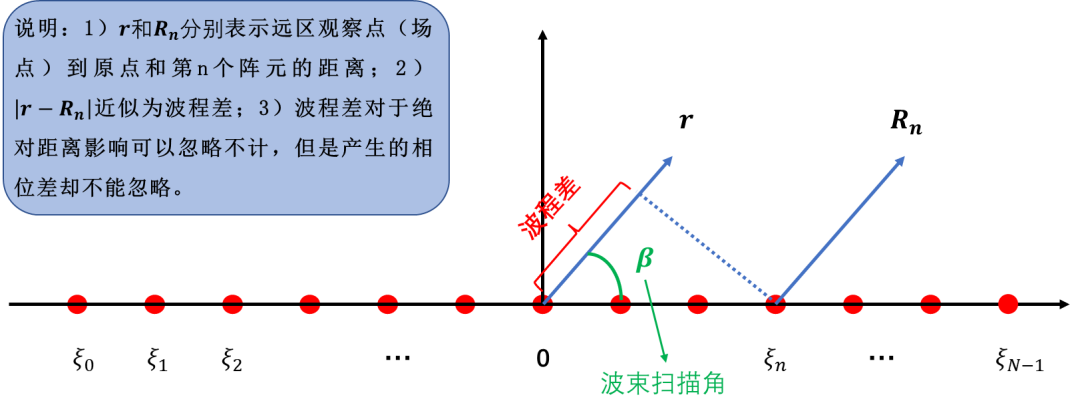
\includegraphics[width=0.8\textwidth]{e1.png}
\caption{相控阵波束扫描原理示意图}
\label{fig:beamscanning}
\end{figure}

\subsection{阵列性能参数}

\textbf{阵列因子 (Array Factor, AF)}：对于一个由 $N$ 个单元组成的均匀线阵，若参考单元位于阵列一端，其阵列因子可表示为：

$$AF(\theta) = \sum_{n=0}^{N-1} I_n e^{j n (kd \cos\theta + \alpha)}$$

其中 $I_n$ 是第 $n$ 个单元的激励电流，本实验中采用均匀幅度激励；$k = 2\pi/\lambda$ 是波数；$d$ 是单元间距；$\alpha$ 是相邻单元的相位差；$\theta$ 是相对于阵列轴的角度。阵列的最终辐射方向图是单个单元方向图与阵列因子的乘积。

\textbf{半功率波束宽度 (HPBW)}：HPBW 是衡量阵列方向图主瓣锐利程度的关键指标，定义为主瓣功率下降到最大值一半时的角宽度。它与阵列的单元数量 $N$、单元间距 $d$ 以及扫描角度 $\theta_0$ 密切相关。通常，阵列的总电气长度 $Nd$ 越大，HPBW 越窄。

\textbf{栅瓣 (Grating Lobes)}：当阵元间距 $d$ 过大时，除了主瓣之外，阵列因子在可见区域（$0^\circ \le \theta \le 180^\circ$）内可能出现与主瓣强度相当的次极大值，即栅瓣。栅瓣会显著降低天线的性能。为了避免栅瓣的出现，单元间距 $d$ 需满足特定条件。

\section{天线阵列参数计算}

本次实验任务旨在设计并仿真一个均匀线阵天线，具体目标如下：

\subsection{无栅瓣条件下的单元间距范围}

由设计要求，当 $\theta_0 = 60^\circ$ 时，阵因子取得最大值，故有：

$$\psi_0 = kd \cos \theta_0 + \beta = \frac{2\pi}{\lambda} d \cos 60^\circ + \beta = 0$$

解得：$\beta = -\frac{\pi}{\lambda}d$

又，要求无栅瓣，故应满足 $-2\pi < \varphi < 2\pi$，即：

$$\begin{cases}
-kd + \beta > -2\pi \\
kd + \beta < 2\pi
\end{cases}$$

带入 $\beta = -\frac{\pi}{\lambda}d$，可得：\textcolor{red}{\textbf{$d \leq \frac{2}{3}\lambda$ 时，不会出现栅瓣。}}

\subsection{单元激励方式的确定}

对于均匀线性阵，其激励幅度为 $I$，相位差为 $\beta = -\frac{\pi}{\lambda}d$。

令 $d = \frac{\lambda}{2} < \frac{2}{3}\lambda$，则天线单元间的步进相位为：

$$\beta = -\frac{\pi}{\lambda}d = -\frac{\pi}{2}rad = -90^\circ$$

故天线阵的单元激励为 $I_m = Ie^{jm\beta} = Ie^{-jm\frac{\pi}{2}}$，其幅度为 \textcolor{red}{$I$}，相位为 \textcolor{red}{\textbf{$-m\frac{\pi}{2}rad$}}。

即：\textcolor{red}{\textbf{幅度为均匀激励，相邻单元相位差 $\beta = -90^\circ$。}}

\subsection{阵列单元数量的确定}

由题意，天线阵的半波带宽为 $13^\circ$。

根据半功率波束宽度公式：

$$\theta_h = \cos^{-1}\left[\cos\theta_0 - 0.443\frac{\lambda}{(L+d)}\right] - \cos^{-1}\left[\cos\theta_0 + 0.443\frac{\lambda}{(L+d)}\right] = 13^\circ$$

解得：$\frac{\lambda}{(L+d)} = 0.2$，即 $L + d = 5\lambda$

因此：

$$N = \frac{L+d}{d} = \frac{5\lambda}{d}$$

令 $d = \frac{\lambda}{2} \leq \frac{2}{3}\lambda$，可得：

$$N = 5 \times 2 = 10$$

即\textcolor{red}{\textbf{阵列单元个数N=10}}。

\clearpage
\section{仿真步骤}

\subsection{新建设计工程}

\begin{enumerate}
\item 运行 HFSS 并新建工程，将工程文件另存为 \textit{Arrary.aedt}。

\item 设置求解类型，在主菜单栏中选择 \keyblue{HFSS}—\keyblue{Solution Type}，在弹出窗口中选择 \keyblue{Modal}，单击 OK，完成设置，如图：

\begin{figure}[H]
\centering
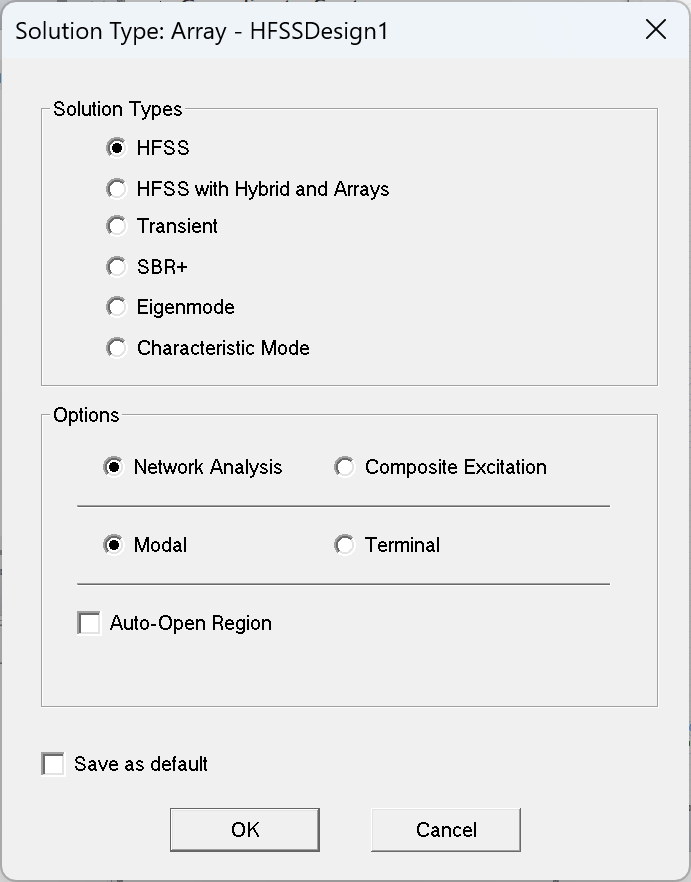
\includegraphics[width=0.5\textwidth]{p1.png}
\caption{设置求解类型}
\label{fig:solution}
\end{figure}

\end{enumerate}

\subsection{添加和定义设计变量}

在主菜单栏中选择 \keyblue{HFSS}—\keyblue{Design Properties}，
打开涉及属性对话框，单击 \keyblue{add} 按钮，打开 \keyblue{AddProperty} 对话框，添加设计变量，如下图：

\begin{figure}[H]
\centering
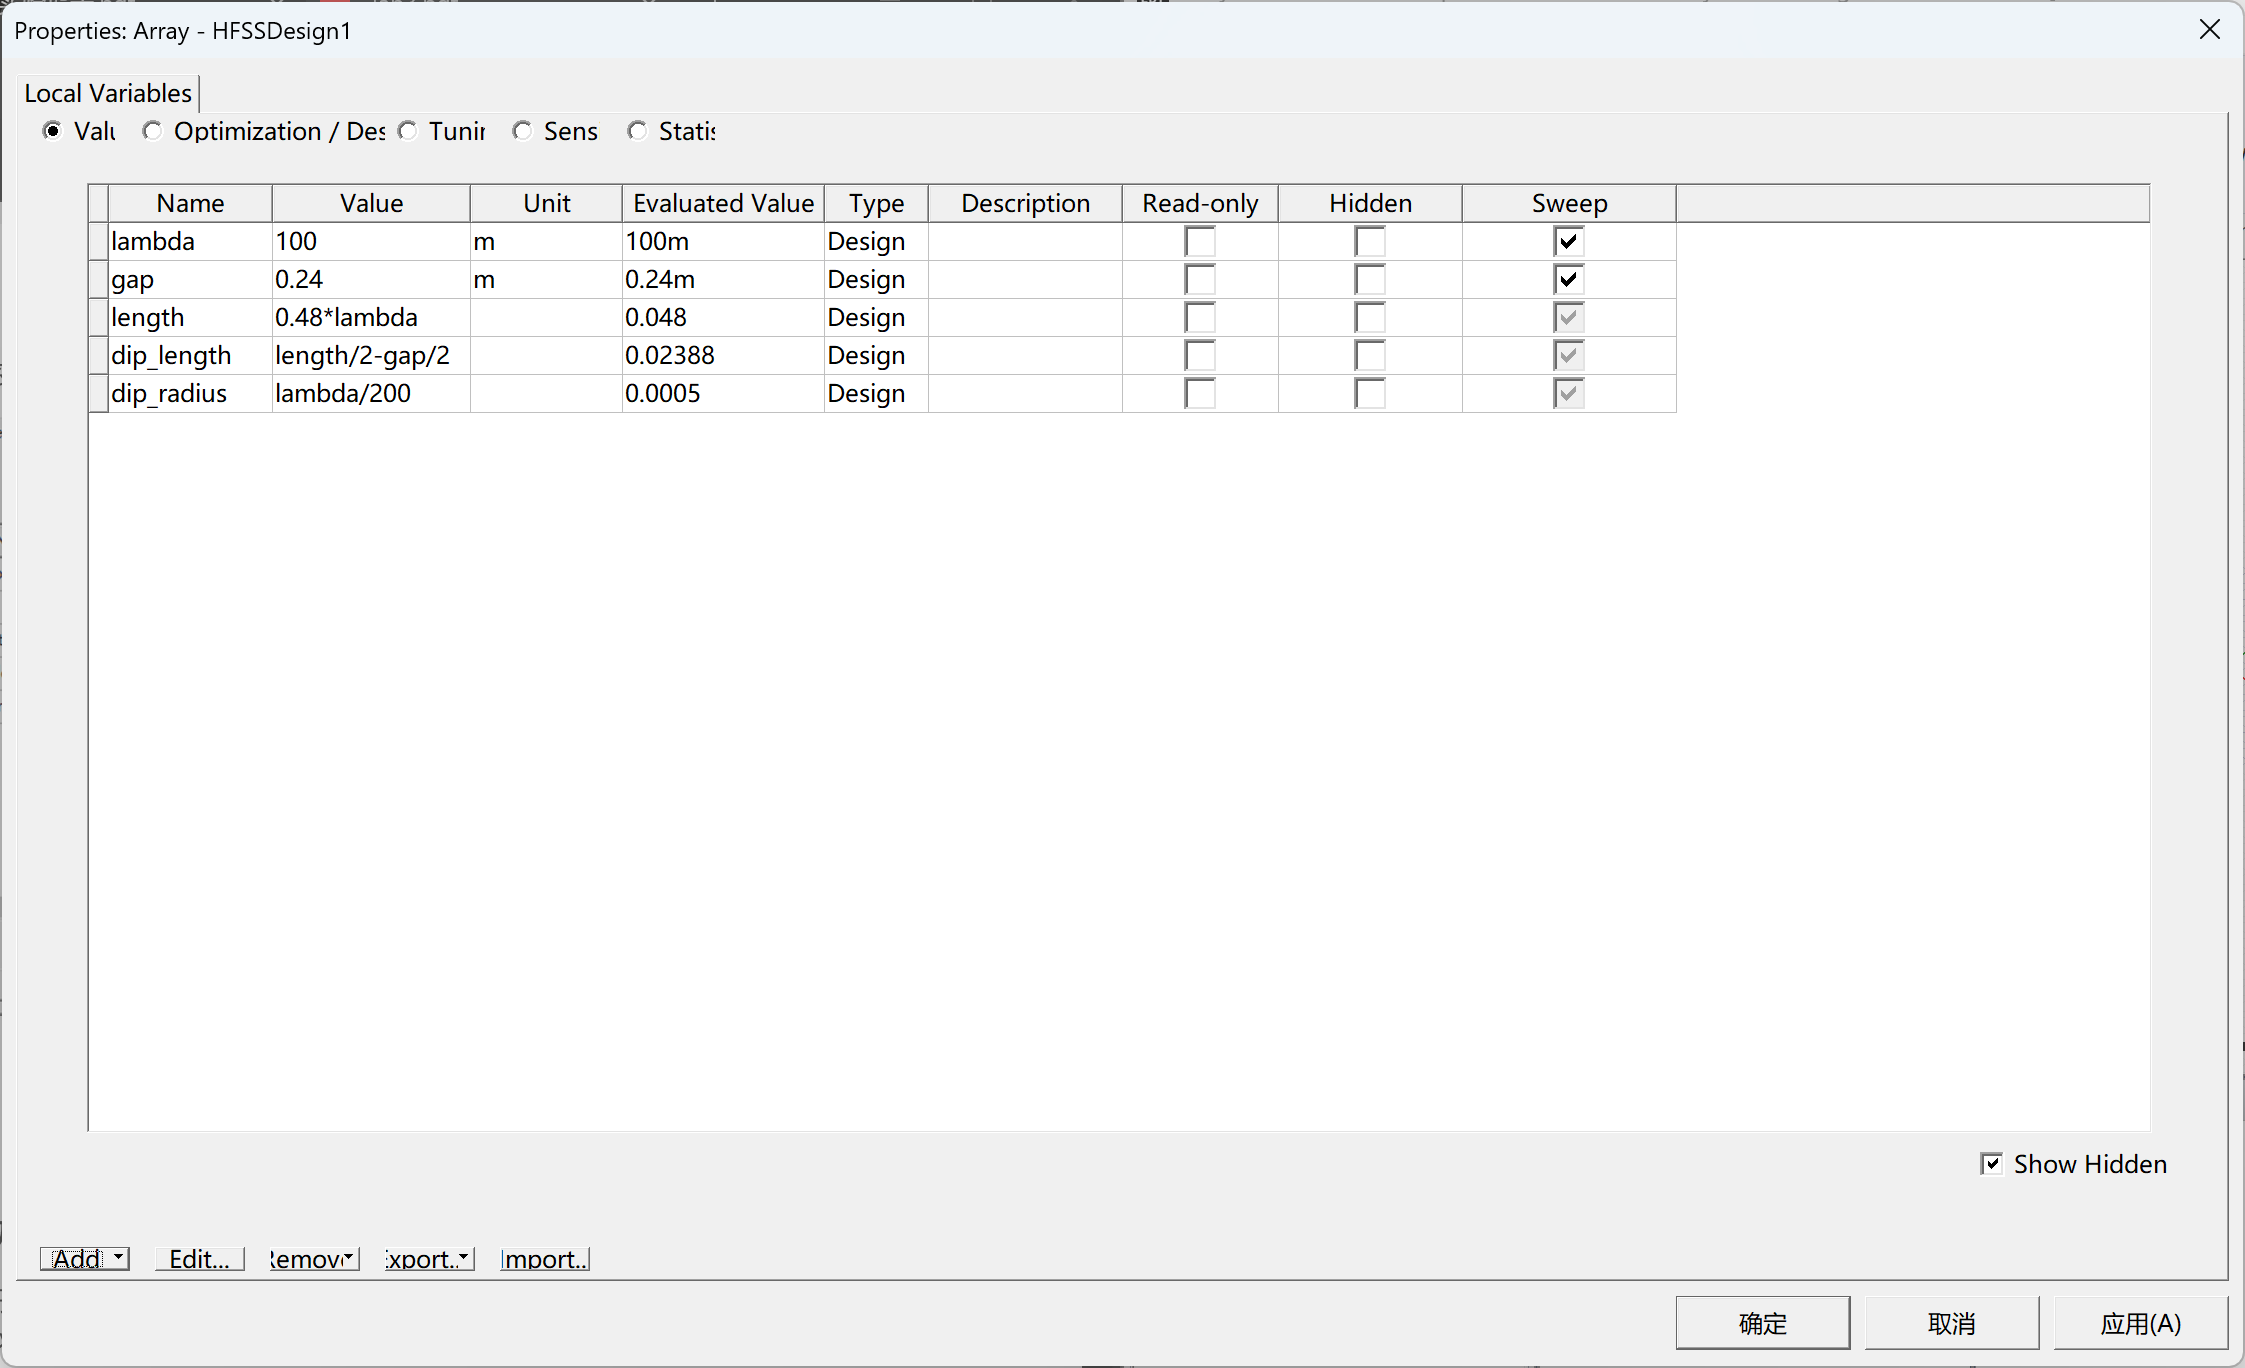
\includegraphics[width=0.8\textwidth]{p2.png}
\caption{添加和定义设计变量}
\label{fig:variables}
\end{figure}

\subsection{偶极子天线建模}

\begin{enumerate}
\item 将工作平面设置为 XZ 平面，并沿 Y 轴绘制圆柱 \keyblue{Dipole}，材质设置为"pec"，中心点设置在 (0,gap/2,0) 处，半径和高度分别设置为 dip-radius 和 dip-length；

\begin{figure}[H]
\centering
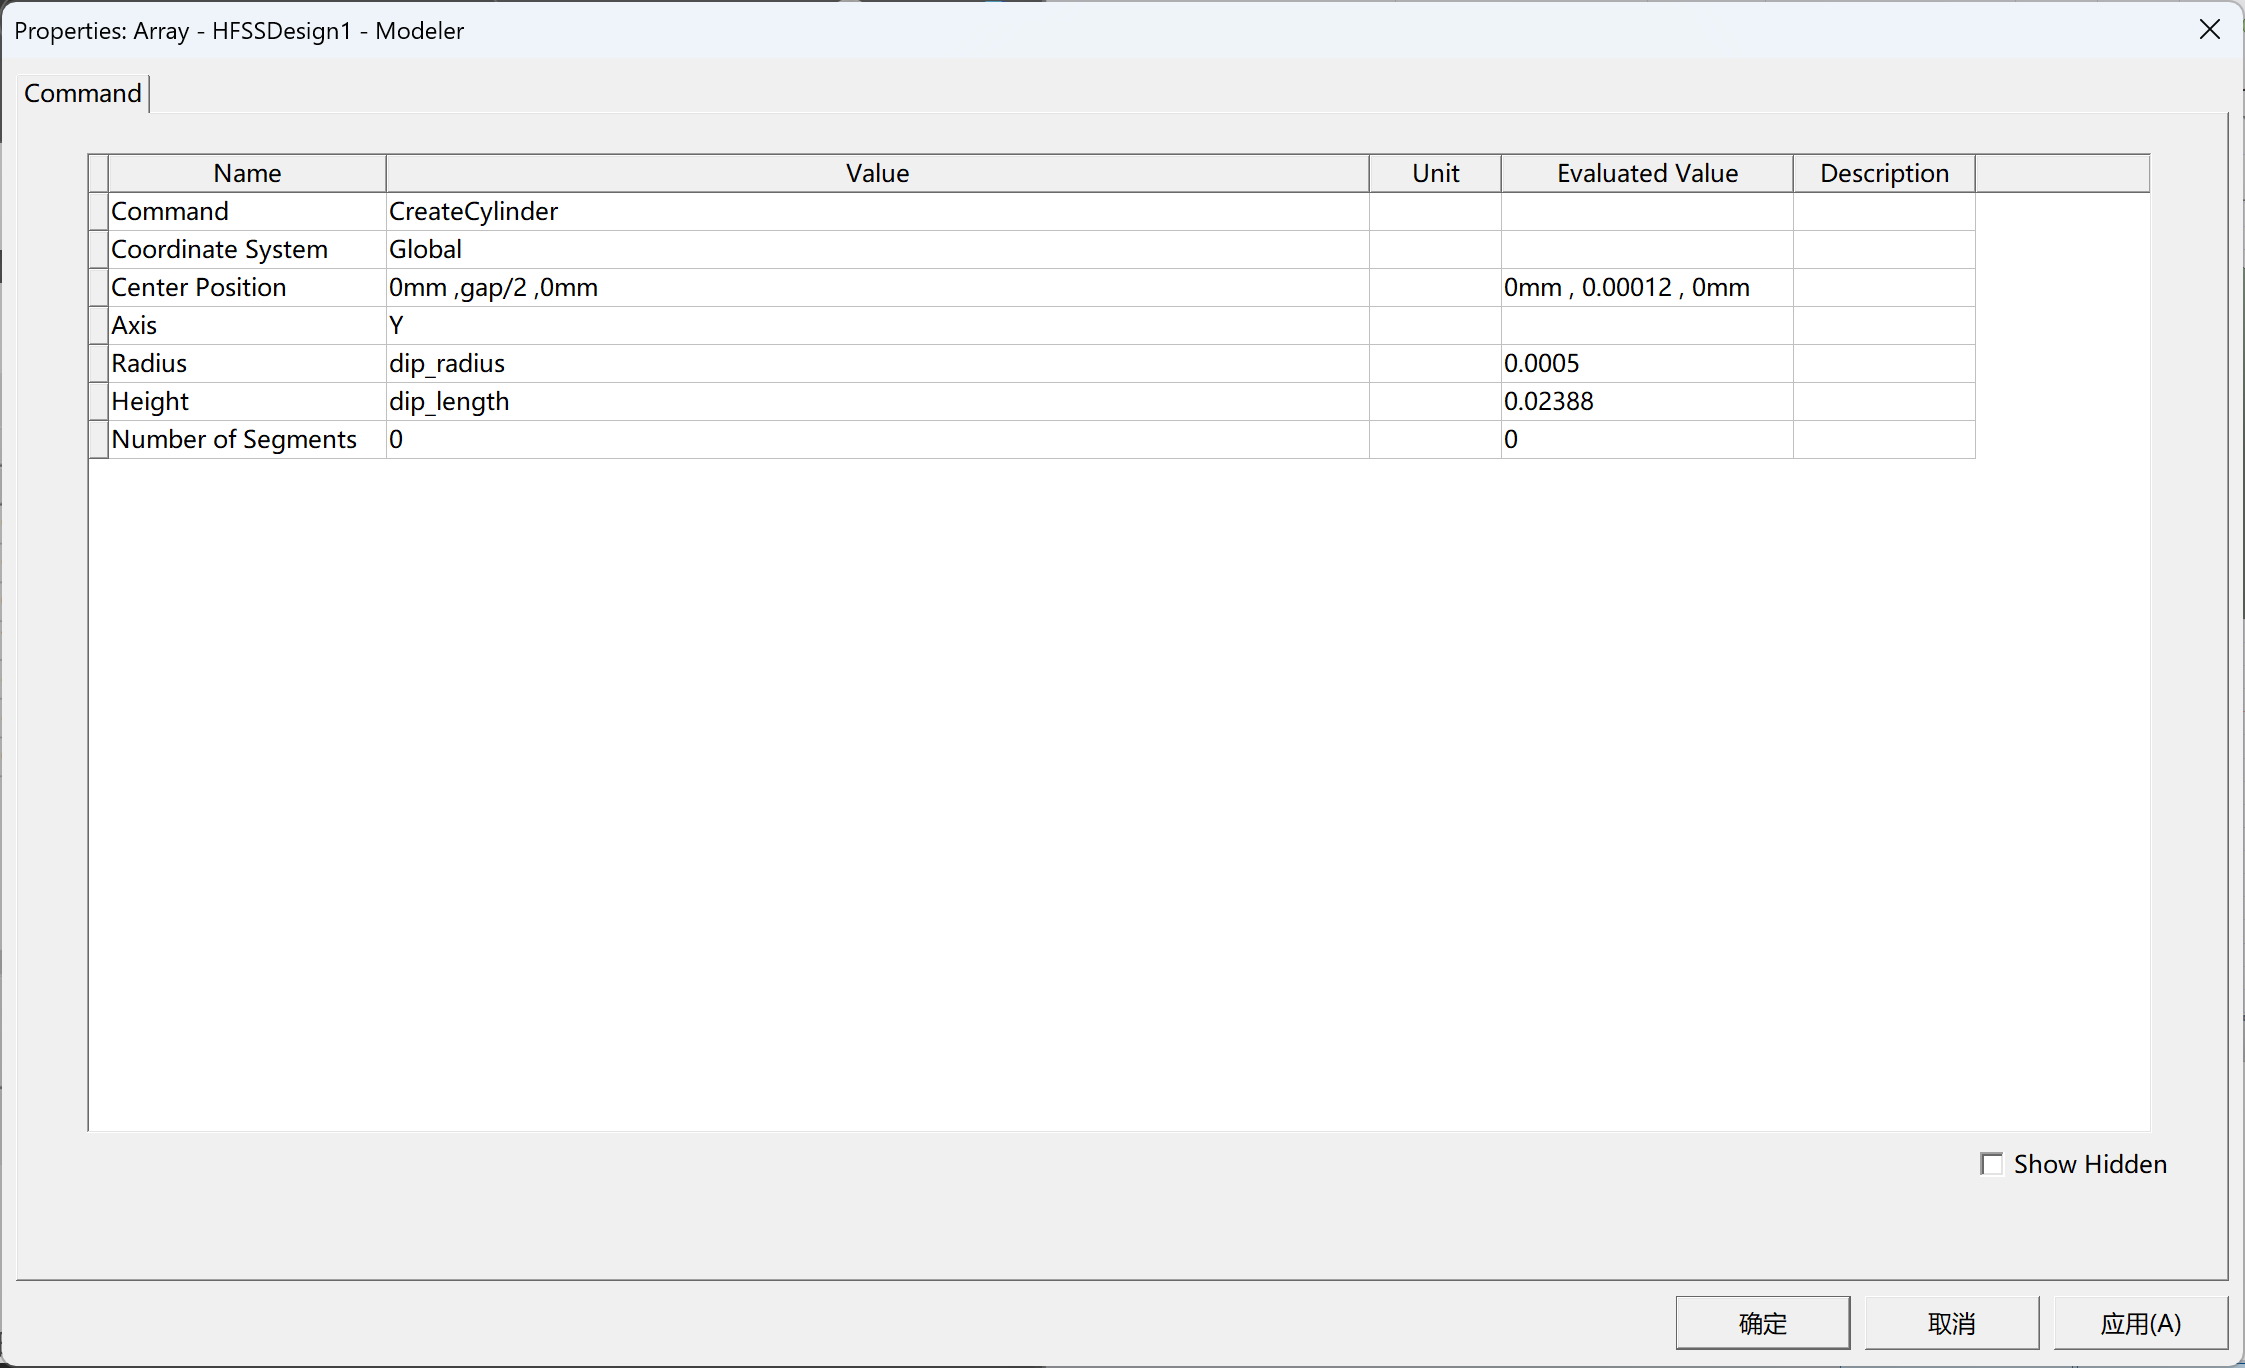
\includegraphics[width=0.8\textwidth]{p4.png}
\caption{偶极子天线模型}
\label{fig:dipole}
\end{figure}

\item 选中创建的圆柱体模型 Dipole，然后从主菜单栏中选择 \keyblue{Edit}—\keyblue{Duplicate}—\keyblue{Around Axis}，执行沿 x 轴旋转 180° 的复制，得到单个偶极子天线。
\end{enumerate}

\begin{figure}[H]
\centering
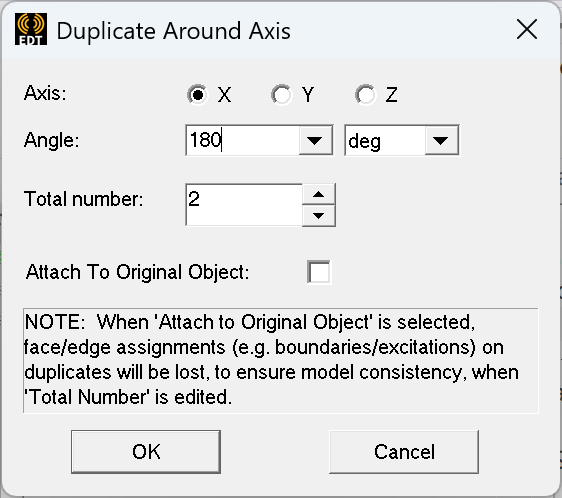
\includegraphics[width=0.5\textwidth]{p5.png}
\caption{复制设置}
\label{fig:duplicate}
\end{figure}

\begin{figure}[H]
\centering
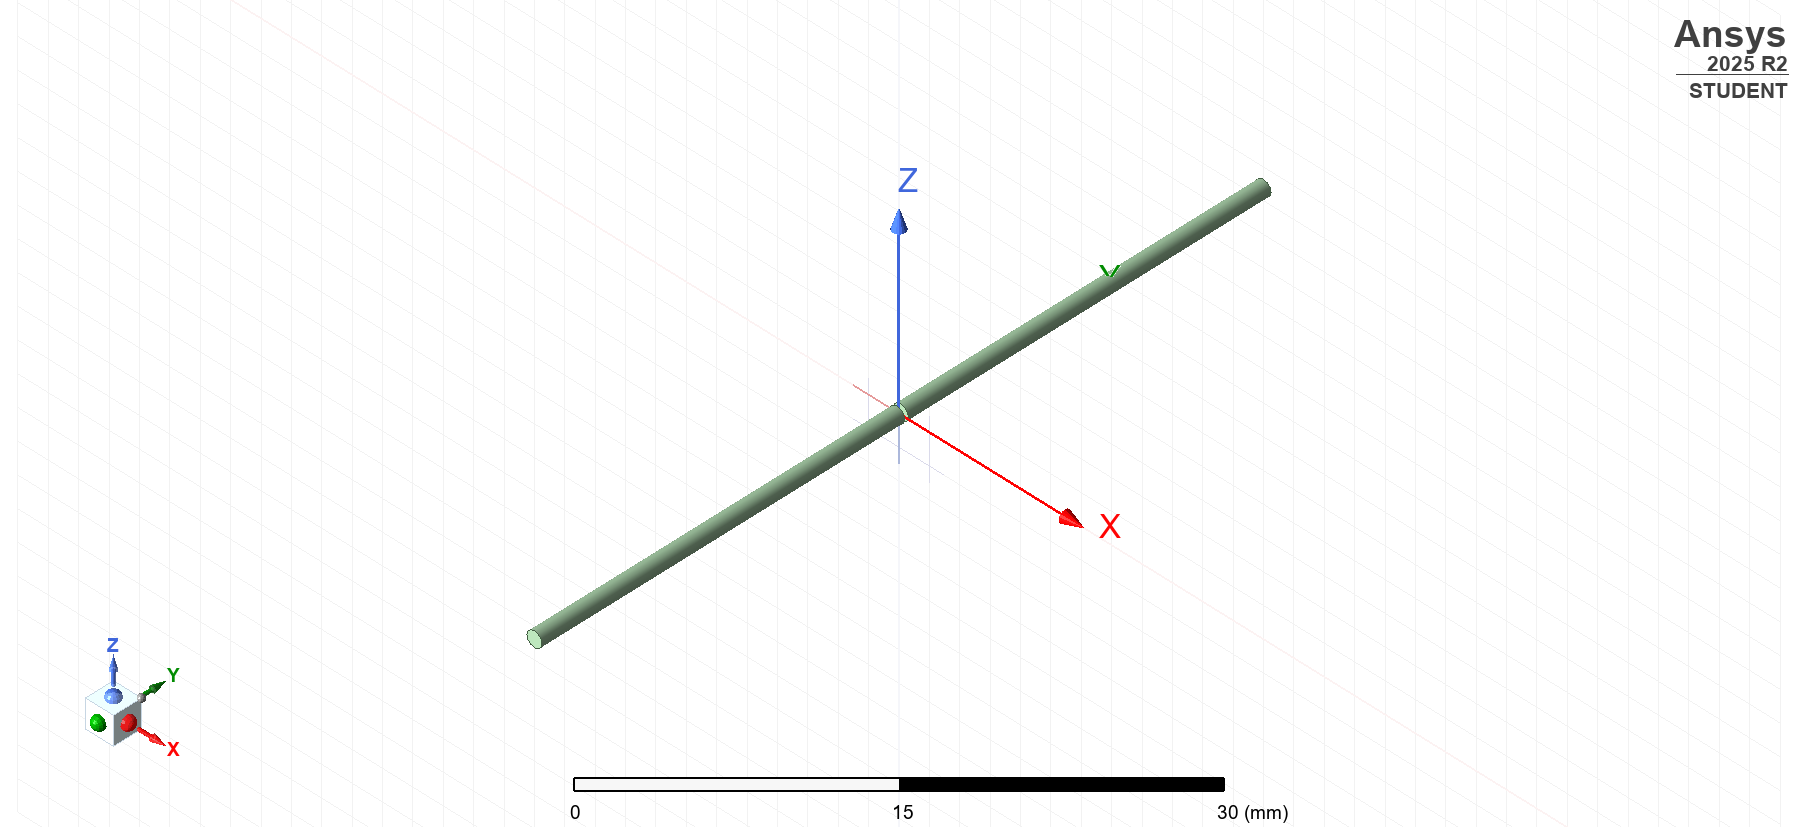
\includegraphics[width=1\textwidth]{p6.png}
\caption{偶极子天线建模图}
\end{figure}

\subsection{端口激励设置}

将工作平面更改为 XY 平面，绘制一个矩形，并设置其中心点在原点，长宽分别为 dip-radius 和 gap，如Figure 6所示，并将其设置为 lumped port，设置如Figure 7所示的激励积分路径：


\begin{figure}[H]
\centering
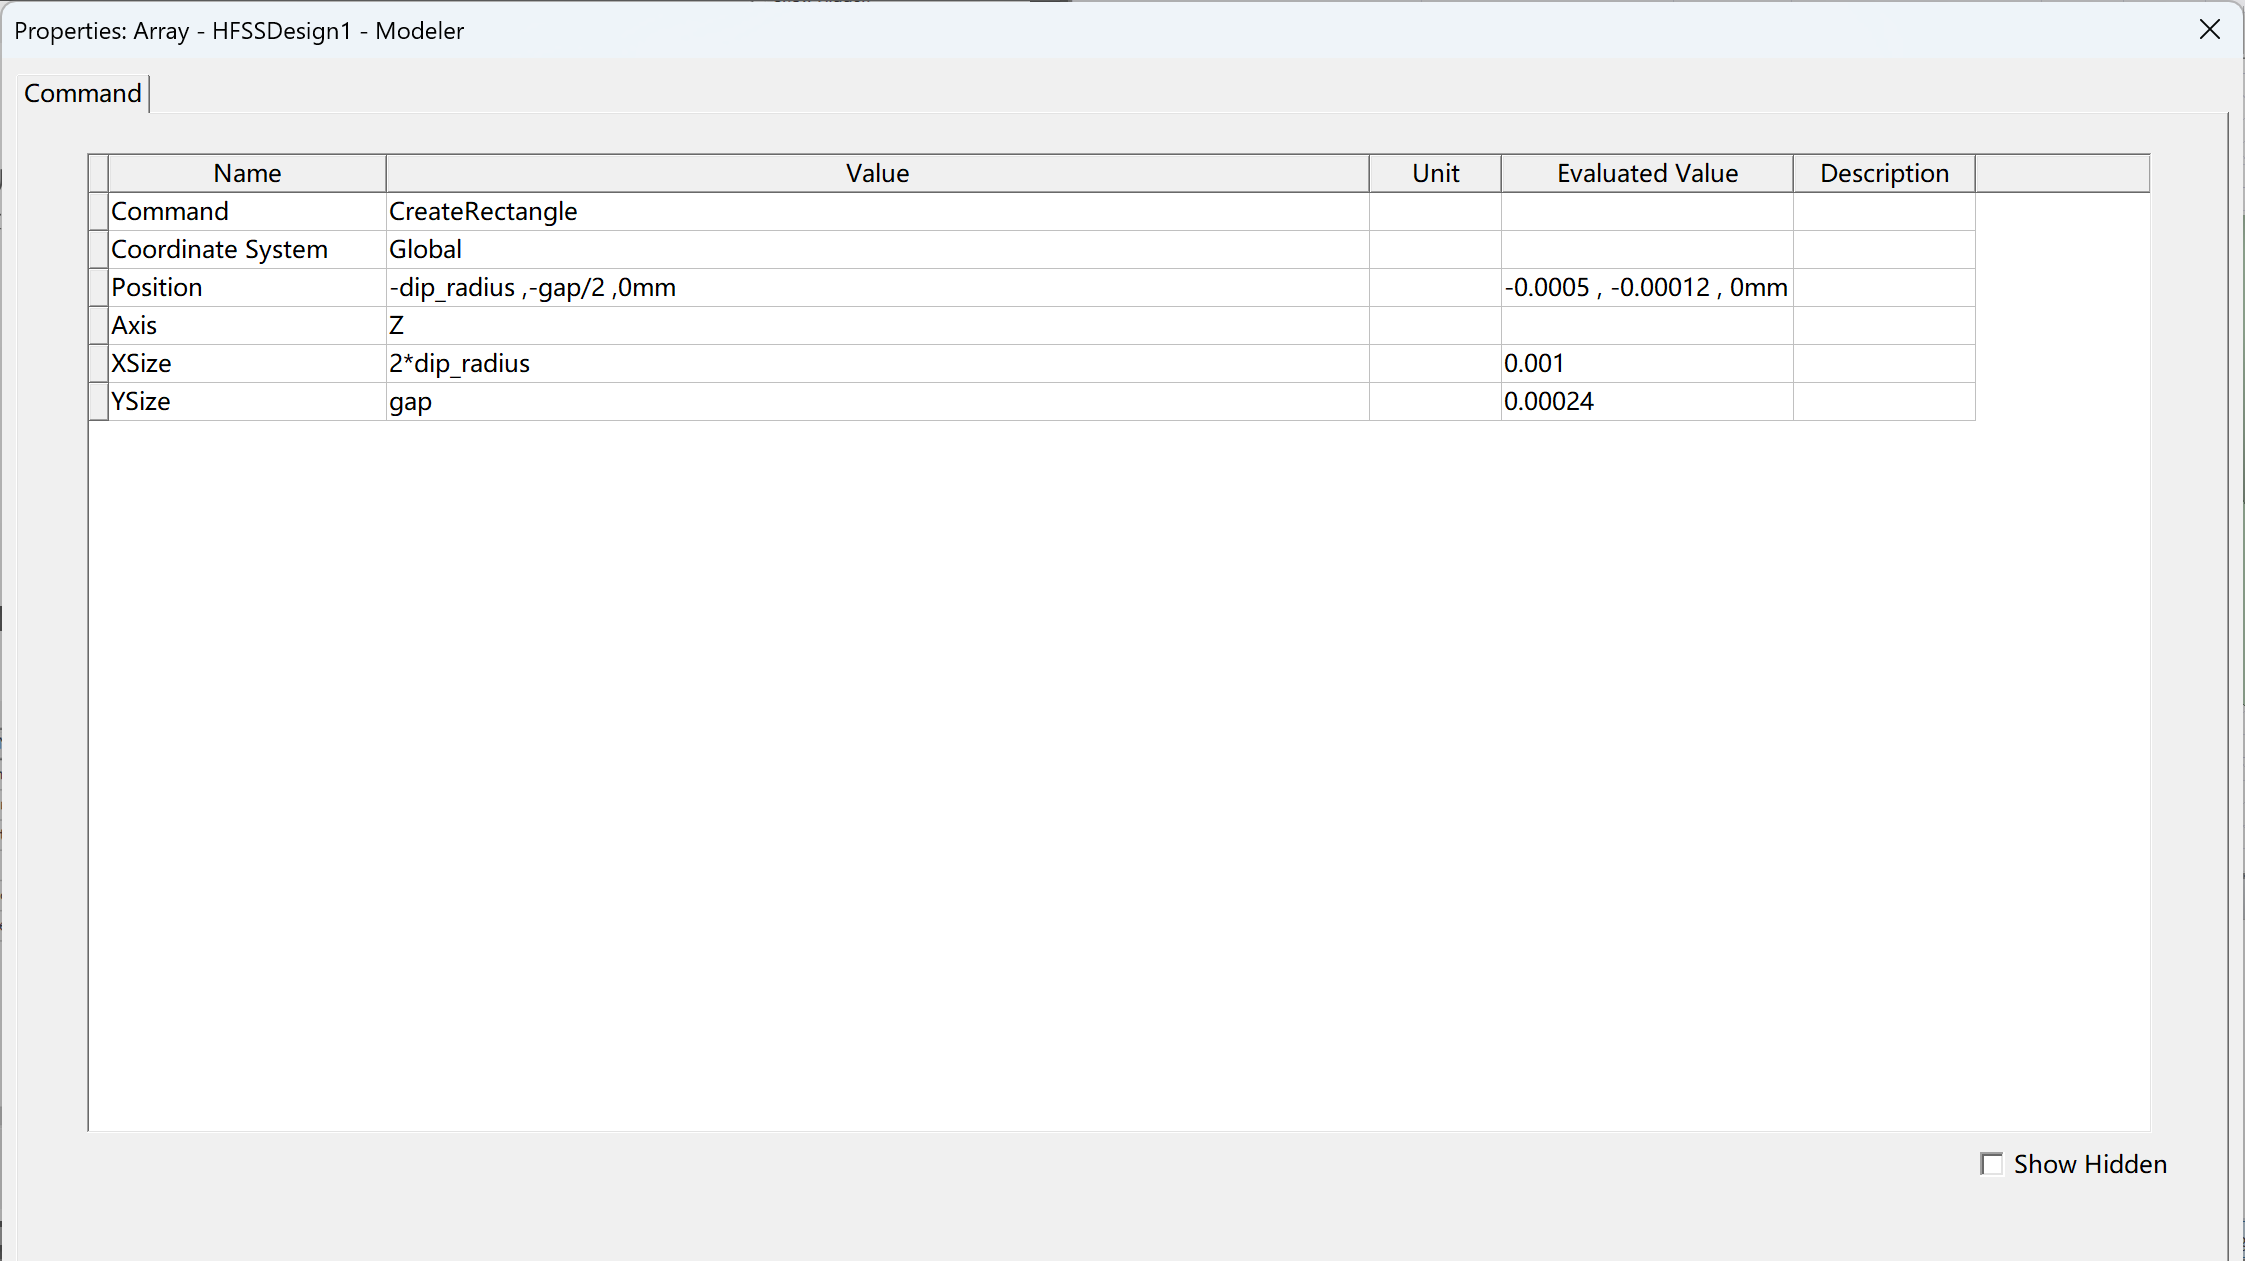
\includegraphics[width=1\textwidth]{p8.png}
\caption{端口模型绘制}
\end{figure}

\begin{figure}[H]
\centering
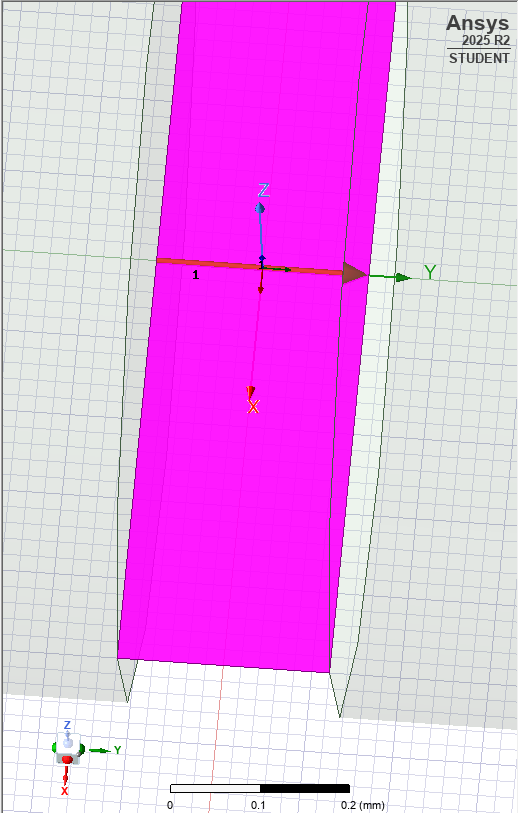
\includegraphics[width=0.5\textwidth]{p10.png}
\caption{端口激励设置}
\label{fig:port}
\end{figure}

\subsection{辐射边界设置}

在菜单栏中选择 \keyblue{Create Region}，并在弹出的窗口中将 Padding Type 改为 Absolute Offset，Value 改为 lambda/4，如下图所示：

\begin{figure}[H]
\centering
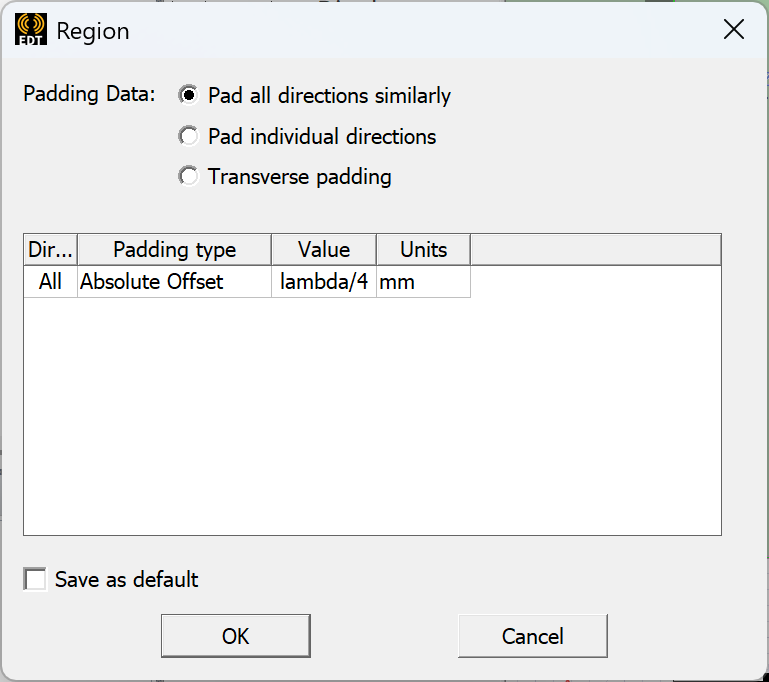
\includegraphics[width=0.5\textwidth]{p11.png}
\caption{辐射边界设置}
\label{fig:region}
\end{figure}

双击操作历史树下,打开属性对话框，将材料改为air,透明度为0.8。
并设置边界模式为 Radiation，最终得到单个偶极子天线的辐射边界。

\begin{figure}[H]
\centering
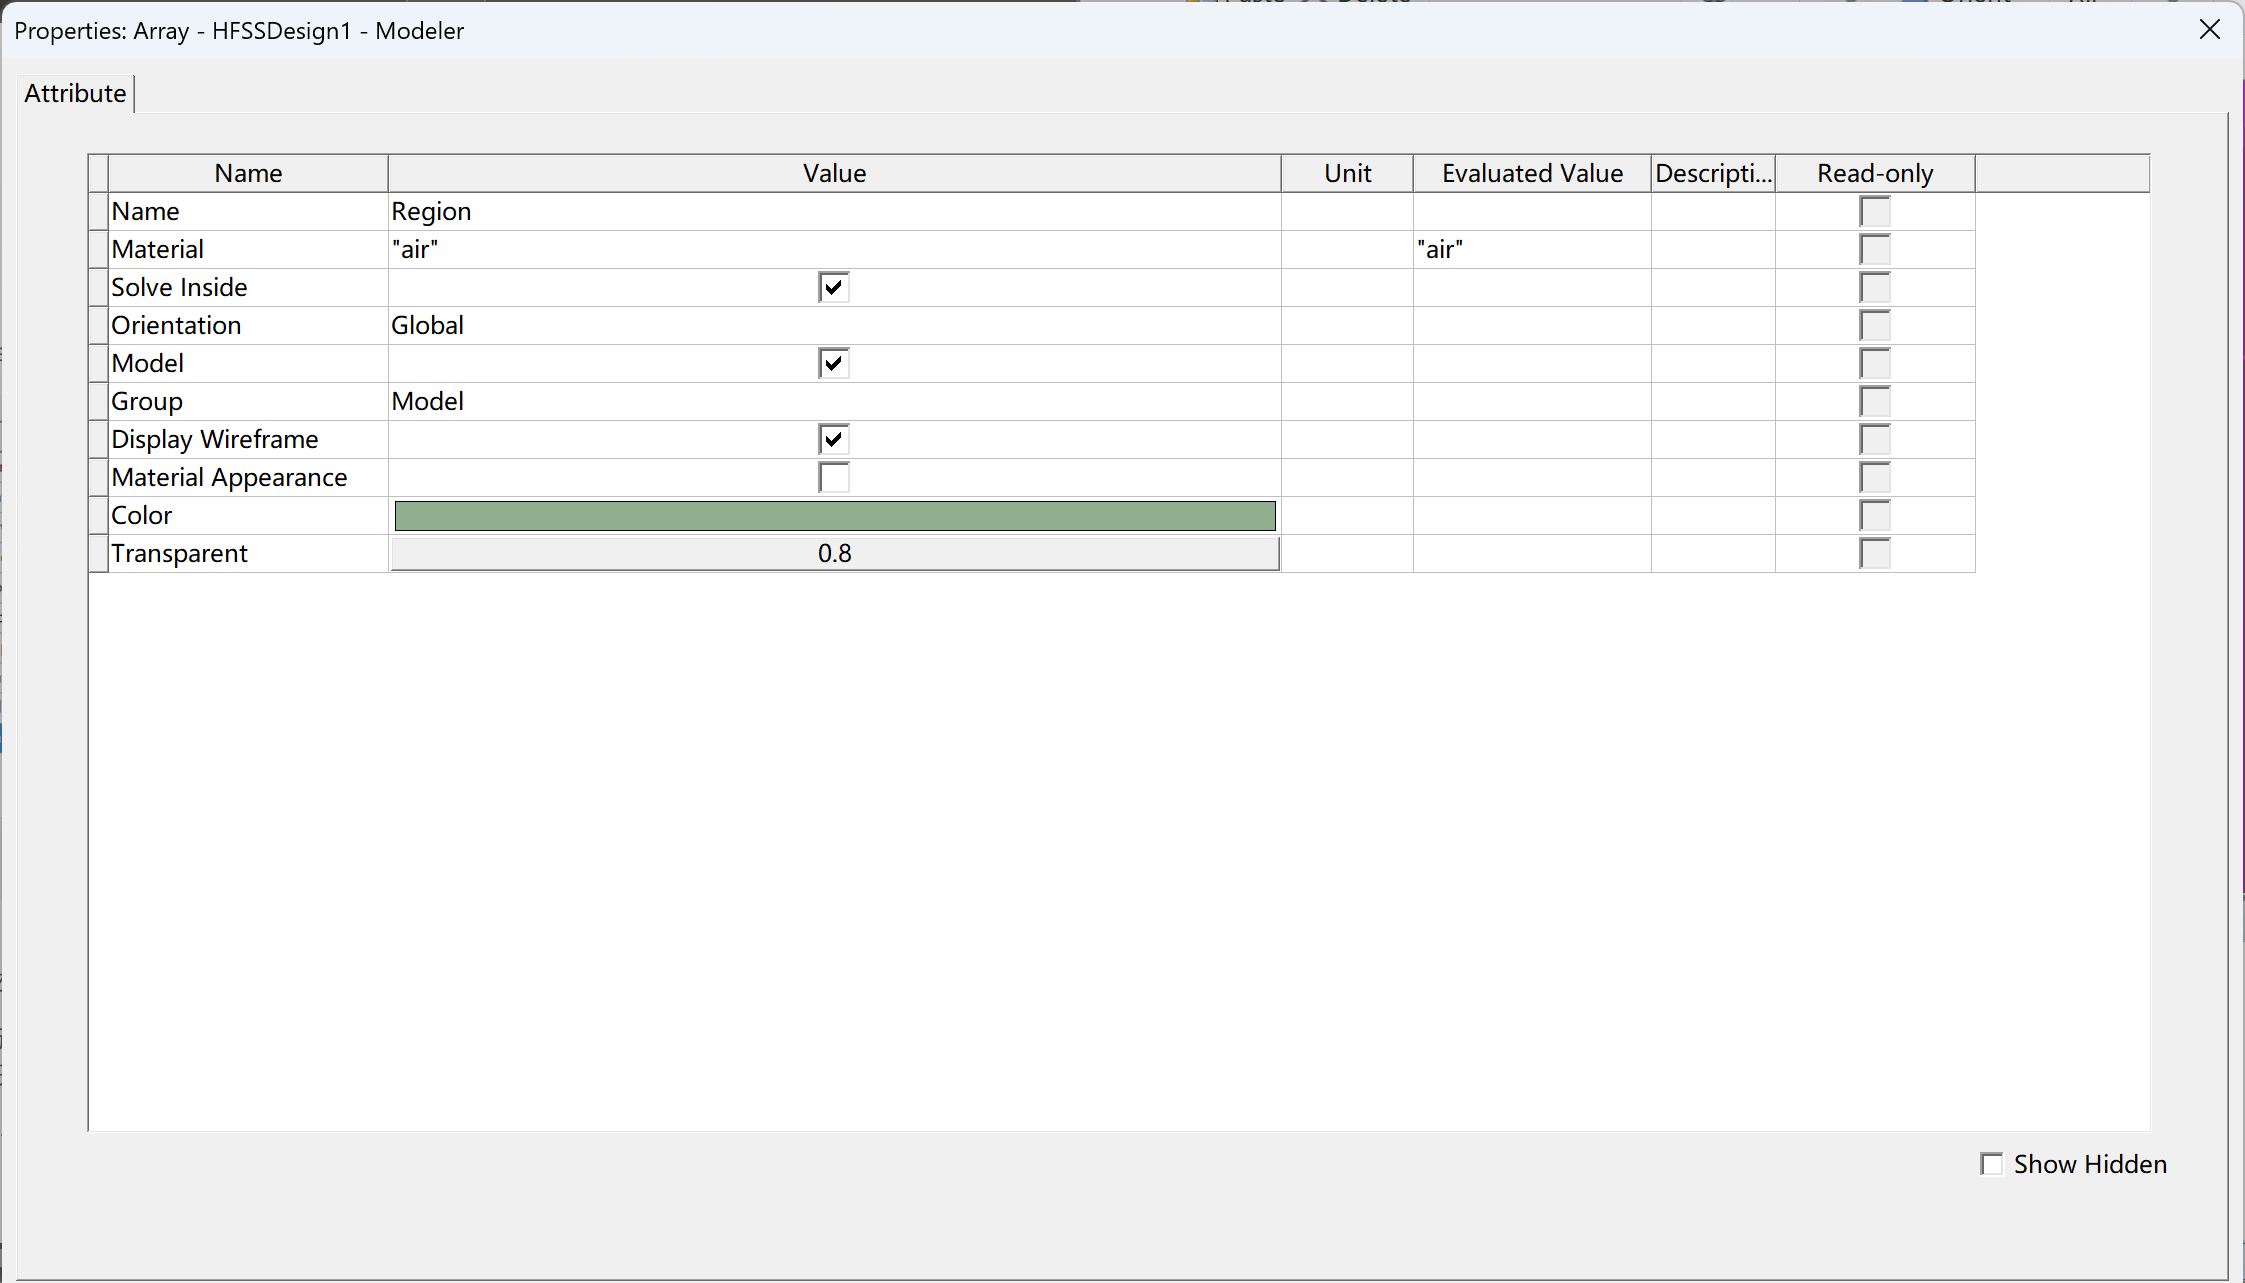
\includegraphics[width=0.9\textwidth]{p12.png}
\caption{设置区域材质}
\label{fig:arraysetup}
\end{figure}

\subsection{天线阵列设置}

在工程树的 Radiation 处选择 \keyblue{Antenna Array Setup}，
并设置基址 z 轴属性，拓展个数为 10 个，间隔为 50mm(0.5*lambda)，天线的步进相位为$-90^\circ$，具体设置如下图所示：
 \begin{figure}[H]
        \centering
        \begin{minipage}[b]{0.48\linewidth}
            \centering
            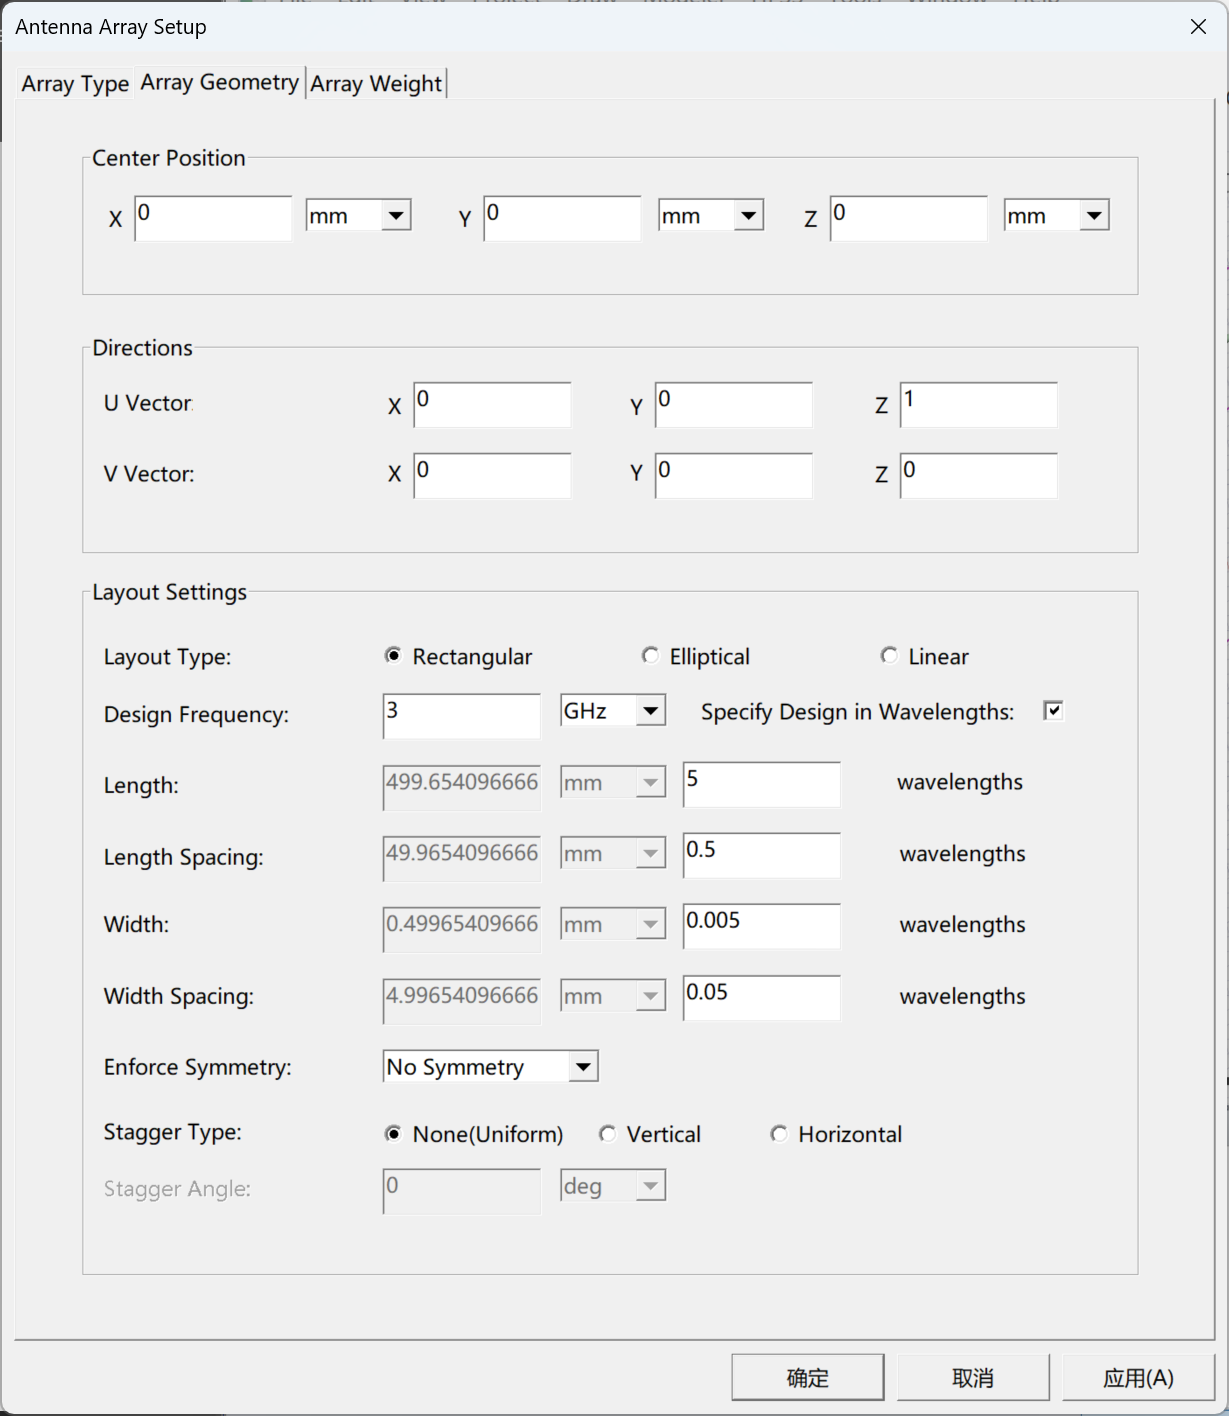
\includegraphics[width=1\textwidth]{p14.png}
             
        \end{minipage}%
        \begin{minipage}[b]{0.48\linewidth}
            \centering
            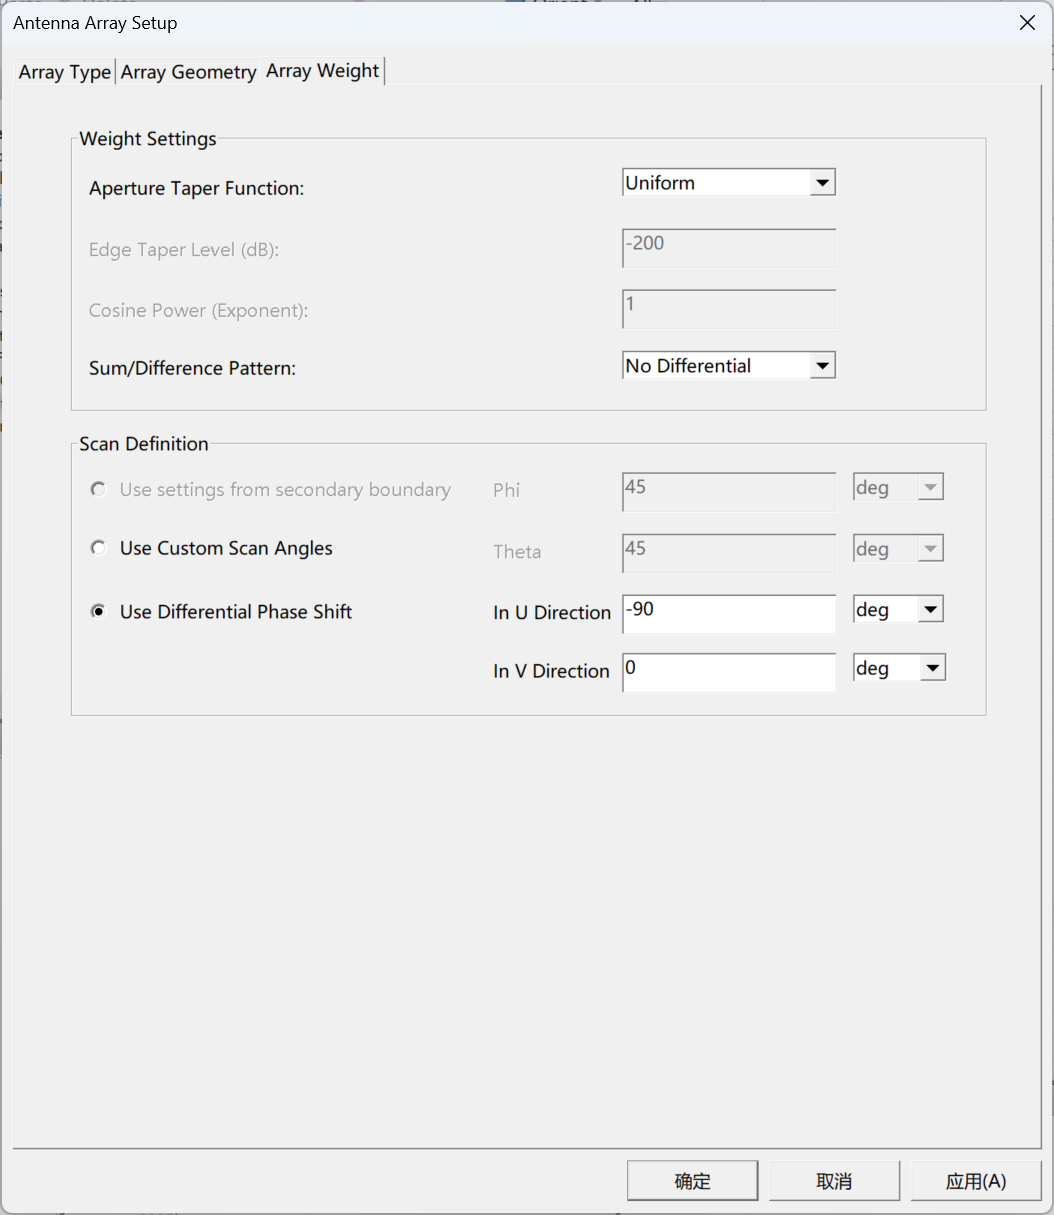
\includegraphics[width=1\textwidth]{p15.png}
        \end{minipage}
        \caption{天线阵列设置}
    \end{figure}

\subsection{仿真设置}

在工程树下的 Analyze 中添加仿真设置，设置仿真频率为 \textbf{3GHz}，并线性扫描 2.5 到 3.5GHz 范围内的 1000 个点。
 \begin{figure}[H]
        \centering
        \begin{minipage}[b]{0.48\linewidth}
            \centering
            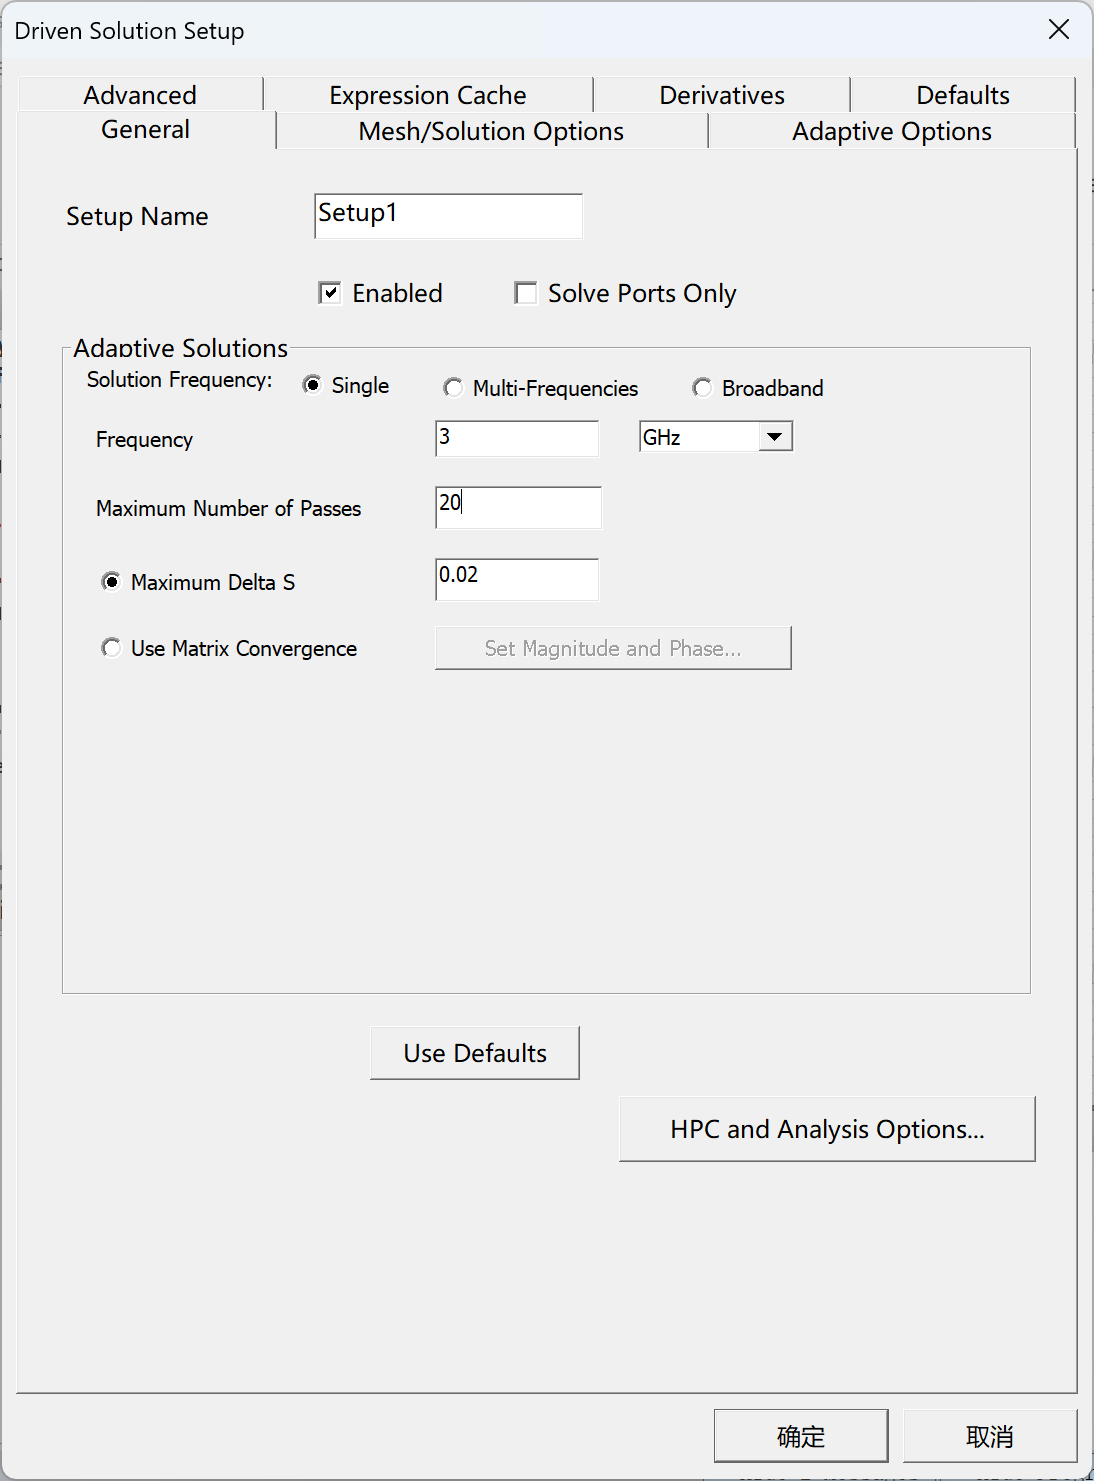
\includegraphics[width=1\textwidth]{p16.png}
             
        \end{minipage}%
        \begin{minipage}[b]{0.48\linewidth}
            \centering
            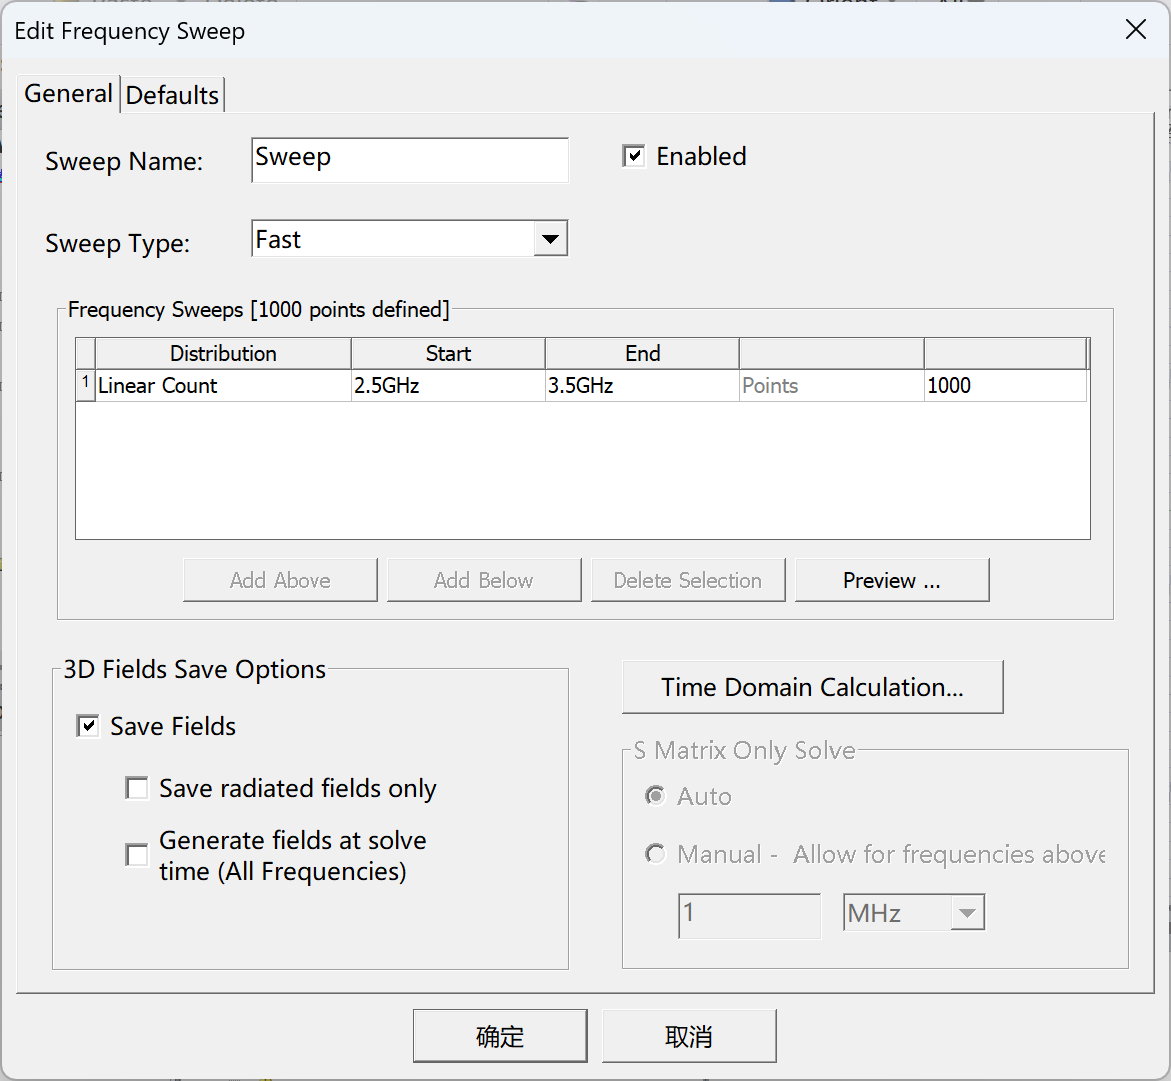
\includegraphics[width=1\textwidth]{p17.png}
        \end{minipage}
        \caption{仿真设置}
    \end{figure}

至此，模型建立完毕，如下所示：

\begin{figure}[H]
\centering
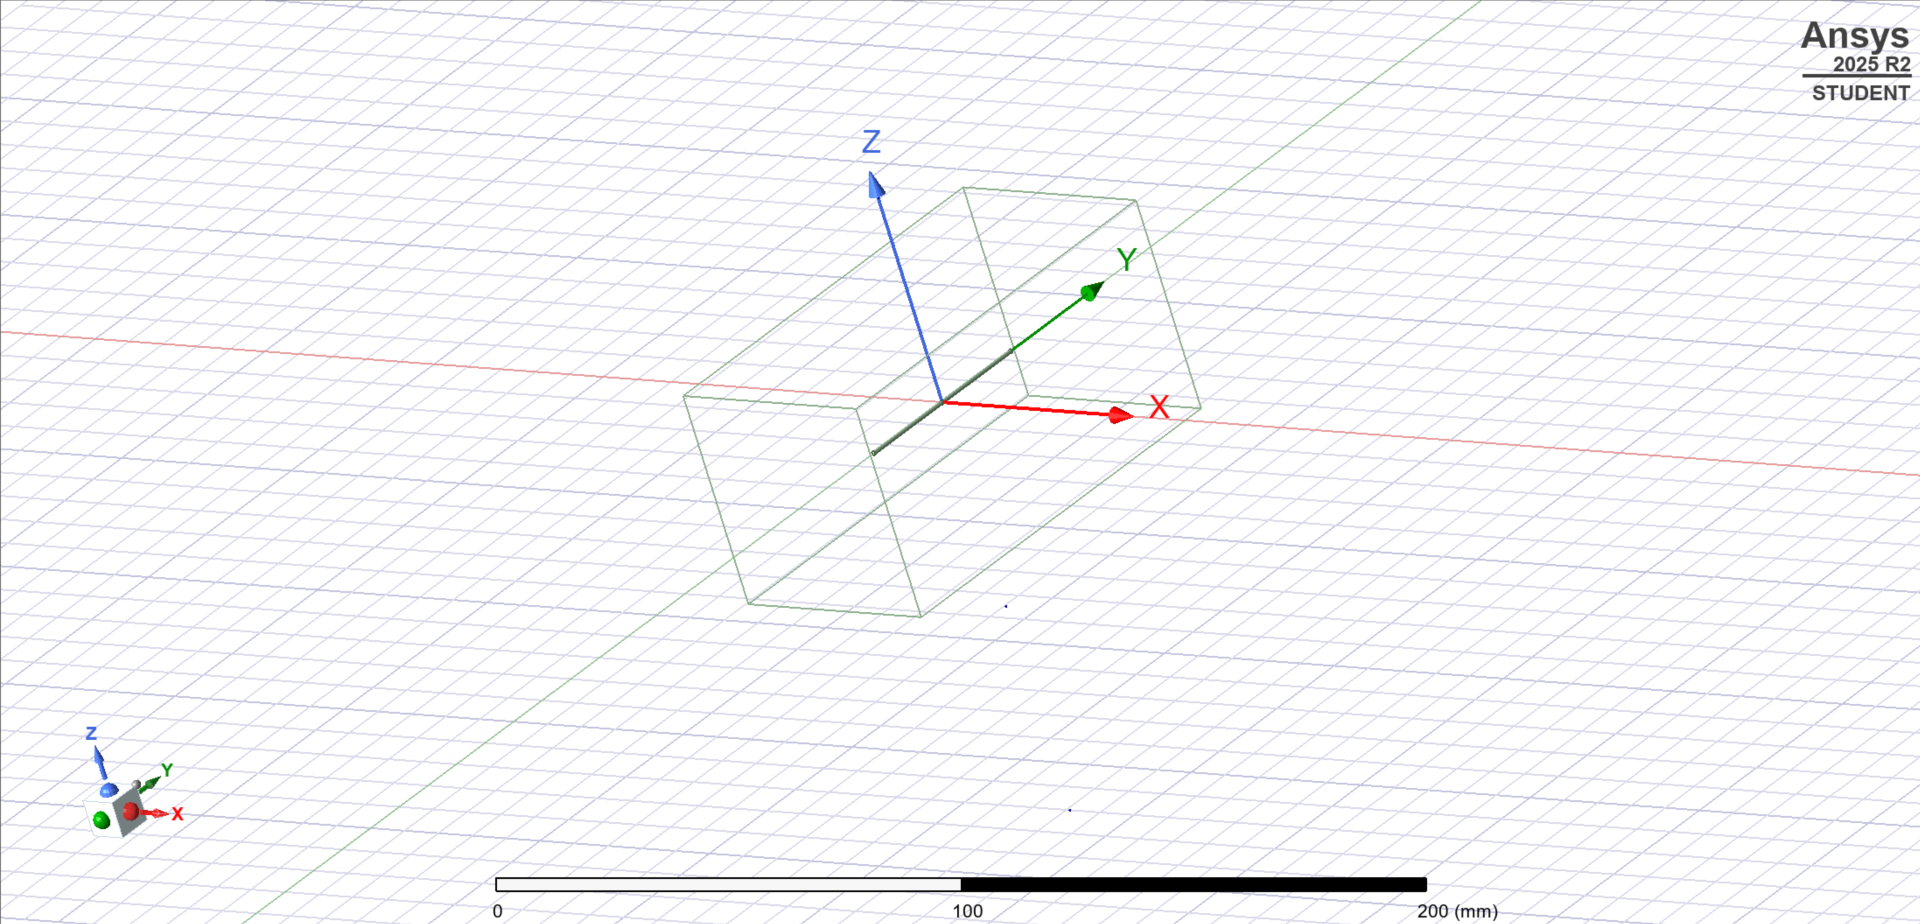
\includegraphics[width=0.5\textwidth]{p19.png}
\caption{仿真模型}
\label{fig:model}
\end{figure}

经检查，设计正确

\begin{figure}[H]
\centering
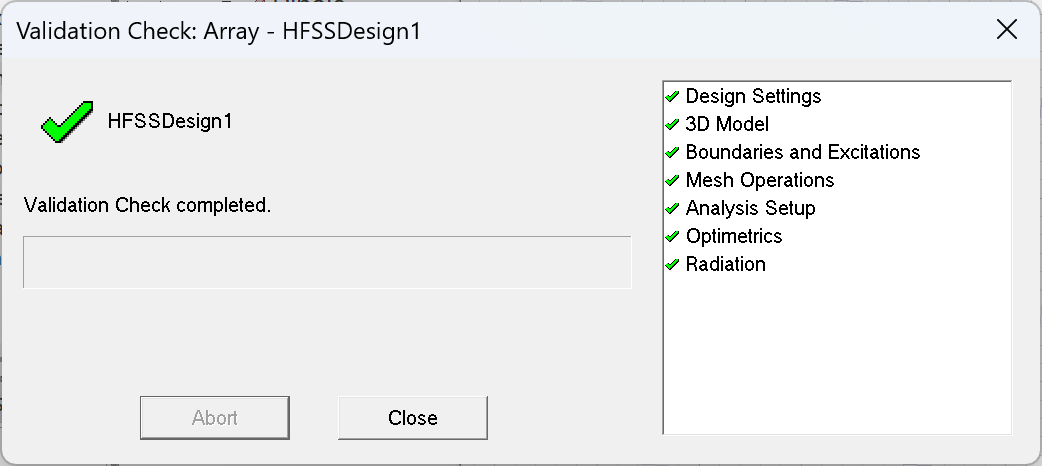
\includegraphics[width=0.5\textwidth]{p18.png}
\caption{仿真模型}
\label{fig:model}
\end{figure}

\section{仿真结果与分析}

\subsection{定义辐射表面}

\begin{enumerate}
    \item 定义辐射表面：右键单击工程树下的 \keyblue{Radiation} 节点，在弹出的快捷菜单中选择 \keyblue{Insert Far Field Setup}-\keyblue{Infinite Sphere}，打开 \keyblue{Far Radiation Sphere Setup}，依次完成以下设置。%：
    
   \begin{figure}[H]
       \centering
       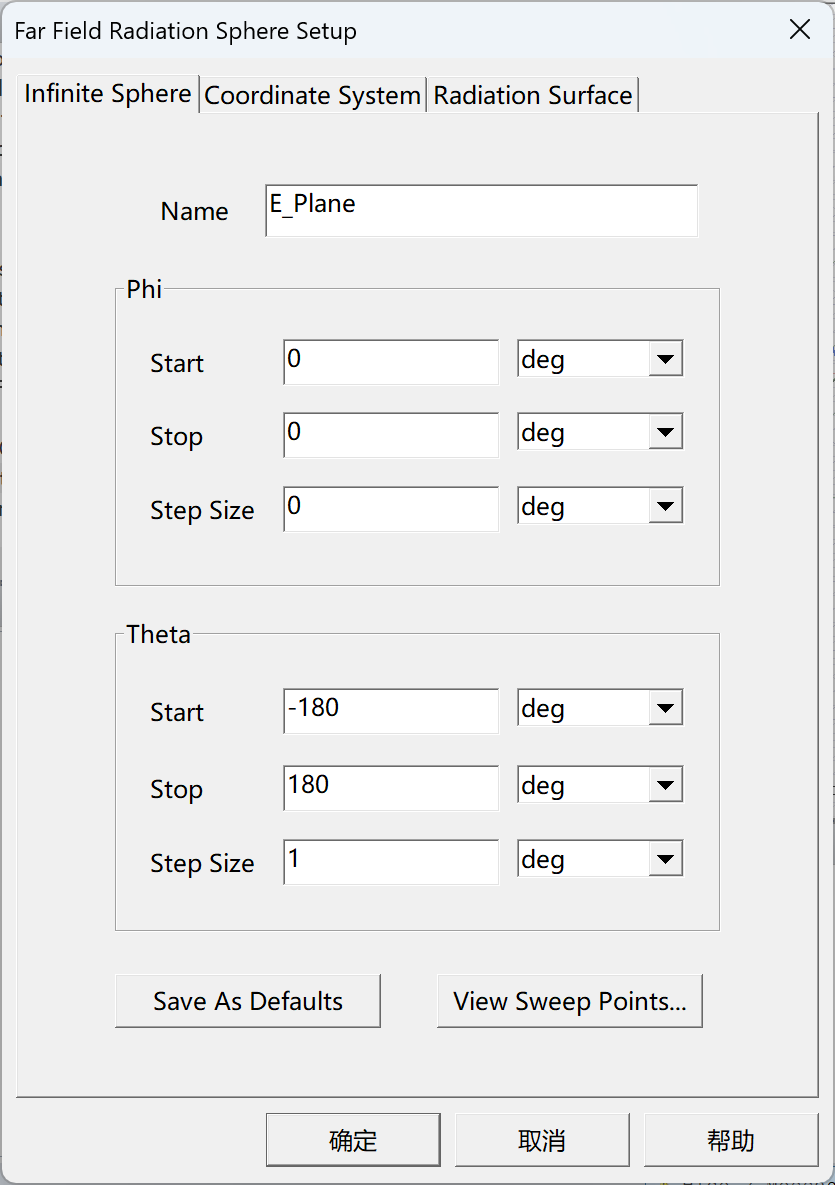
\includegraphics[width=0.32\textwidth]{p20.png}
       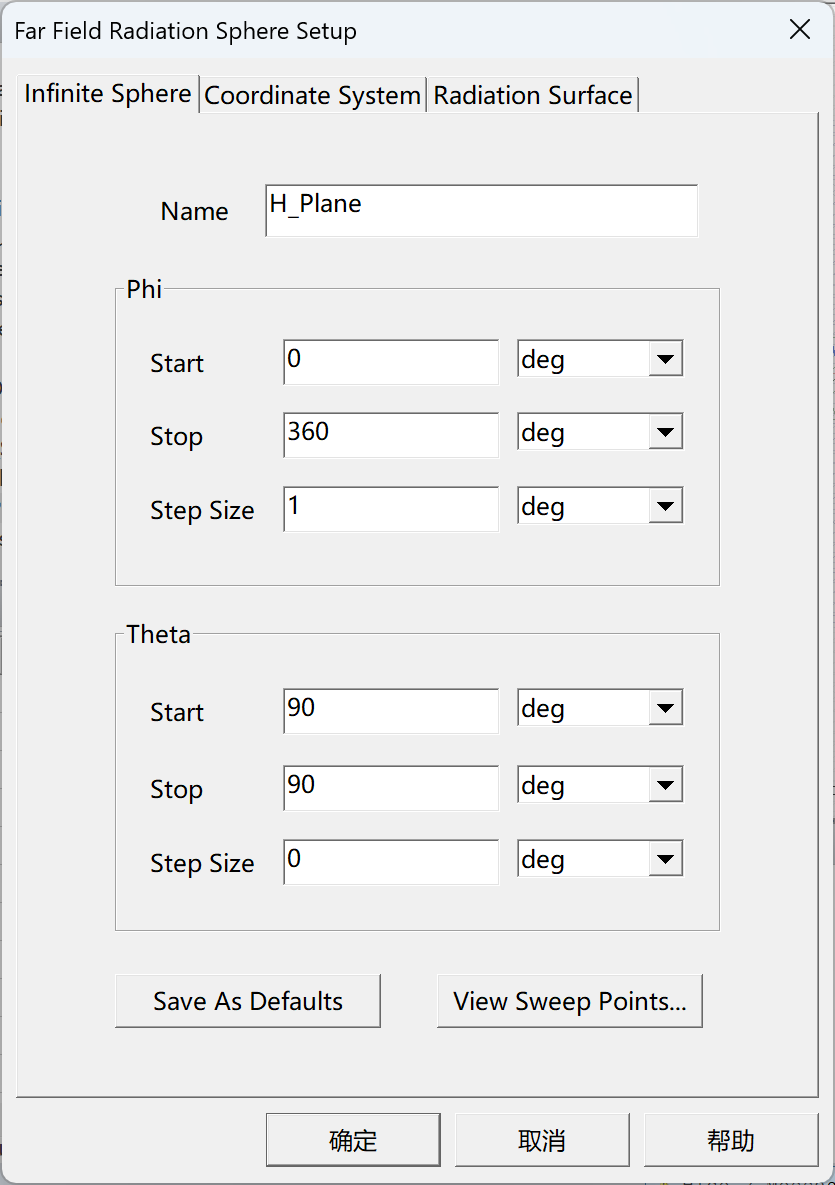
\includegraphics[width=0.32\textwidth]{p21.png}
       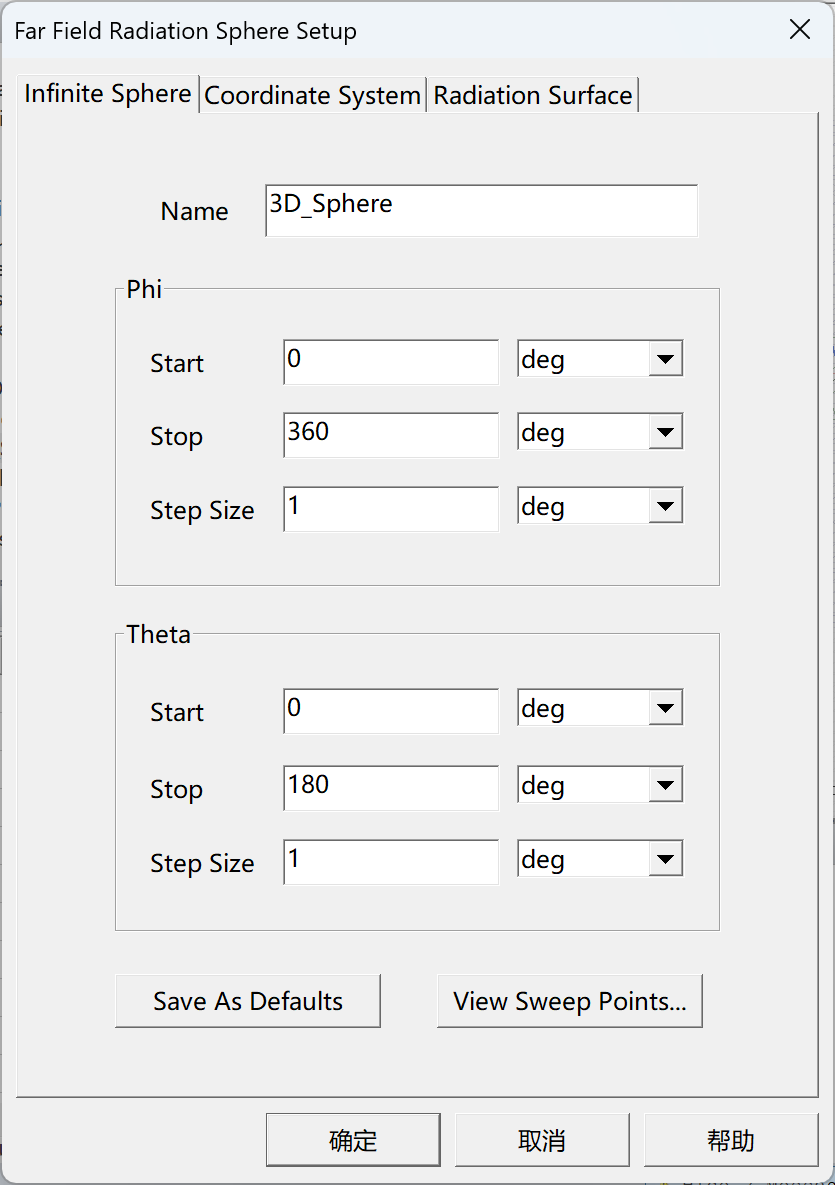
\includegraphics[width=0.32\textwidth]{p22.png}
       \caption{远场辐射球面设置}
       \label{fig:far_field_setup}
   \end{figure}
\end{enumerate}

\subsection{XZ 平面辐射方向图}

根据如下设置，生成极坐标系下天线的 XZ 面增益方向图

\begin{figure}[H]
\centering
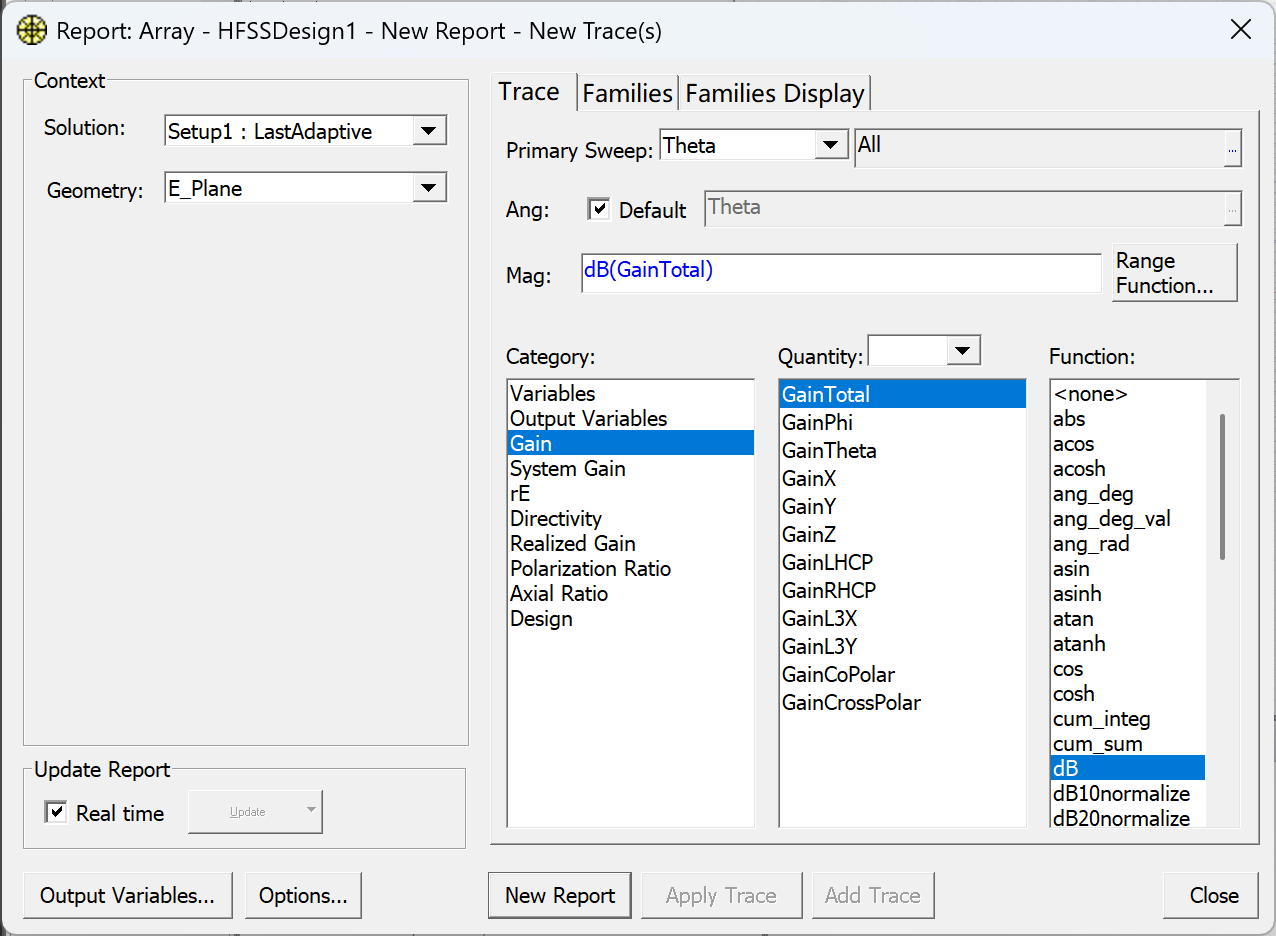
\includegraphics[width=0.6\textwidth]{p23.png}
\caption{XZ 平面辐射方向设置}
\end{figure}

\begin{figure}[H]
\centering
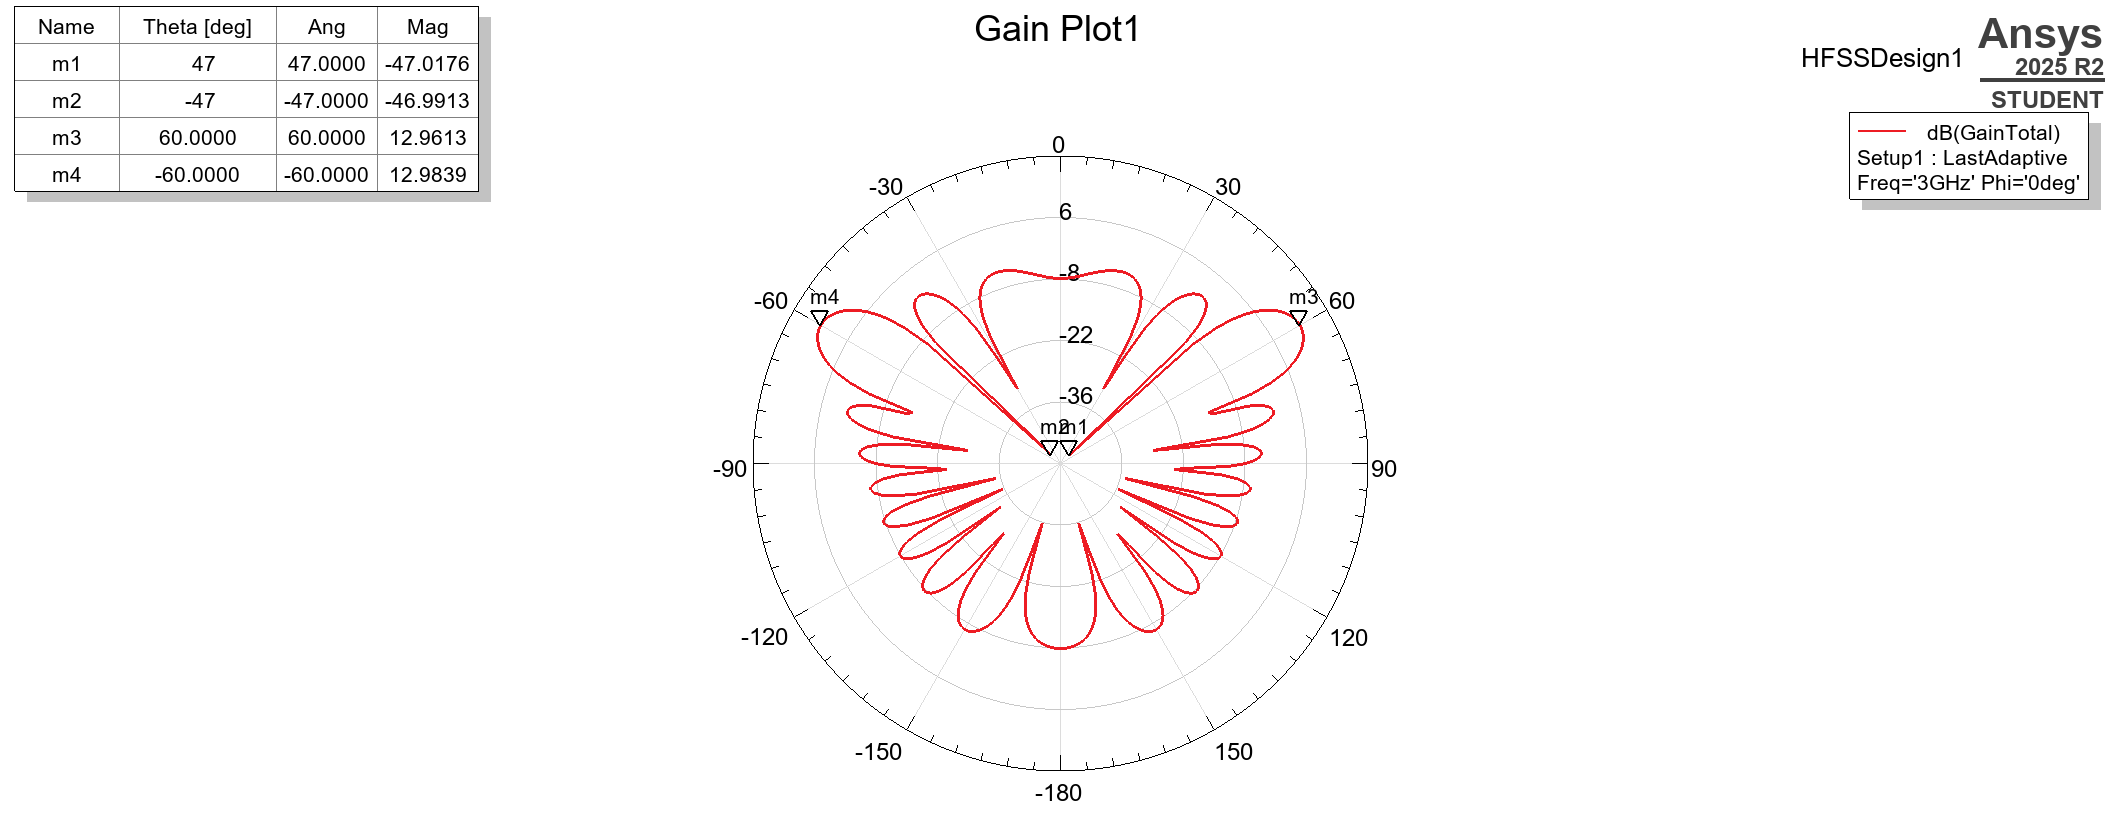
\includegraphics[width=1\textwidth]{p24.png}
\caption{XZ 平面辐射方向图}
\label{fig:xz_pattern}
\end{figure}

从 XZ 平面的辐射方向图中可以看出，天线阵主瓣成功扫描至 $60^\circ$ 方向，获得了约 12.98 dB 的最大增益，验证了设计的正确性。

\subsection{XY 平面辐射方向图}

根据如下设置，生成极坐标系下天线的 XY 面增益方向图

\begin{figure}[H]
\centering
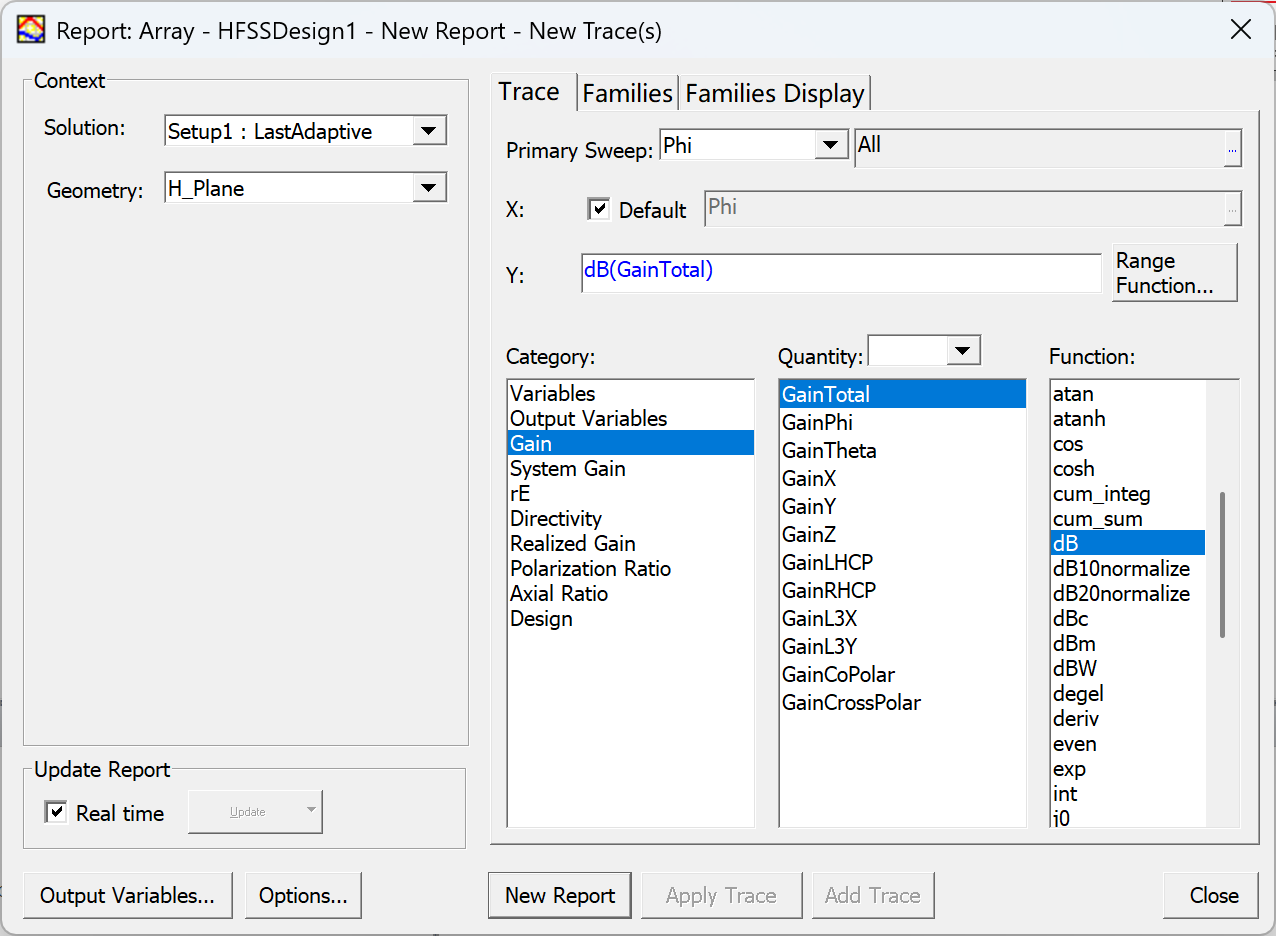
\includegraphics[width=0.6\textwidth]{p25.png}
\caption{XY 平面辐射方向设置}
\end{figure}

\begin{figure}[H]
\centering
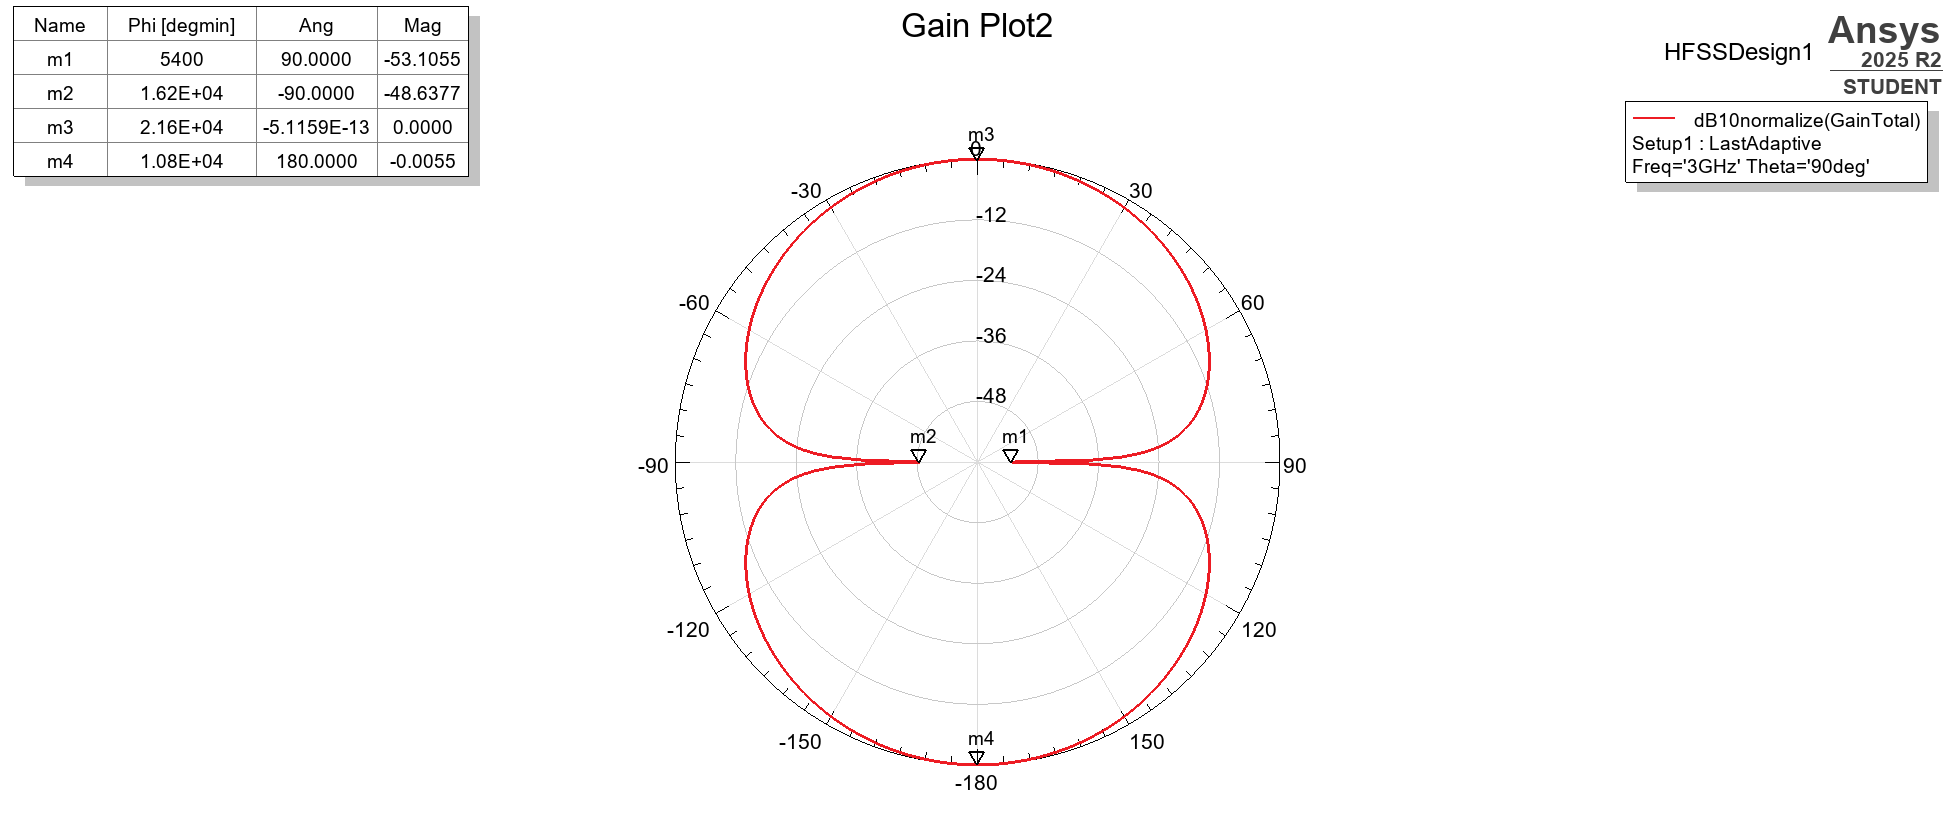
\includegraphics[width=1\textwidth]{p27.png}
\caption{XY 平面辐射方向图}
\label{fig:xy_pattern}
\end{figure}

在 XY 平面上，天线阵列的方向图接近全向，在 XY 方向上没有明显的指向性，这与偶极子天线的固有特性一致。

\subsection{3D 辐射方向图}

根据如下设置，生成天线的 3D 增益方向图

\begin{figure}[H]
\centering
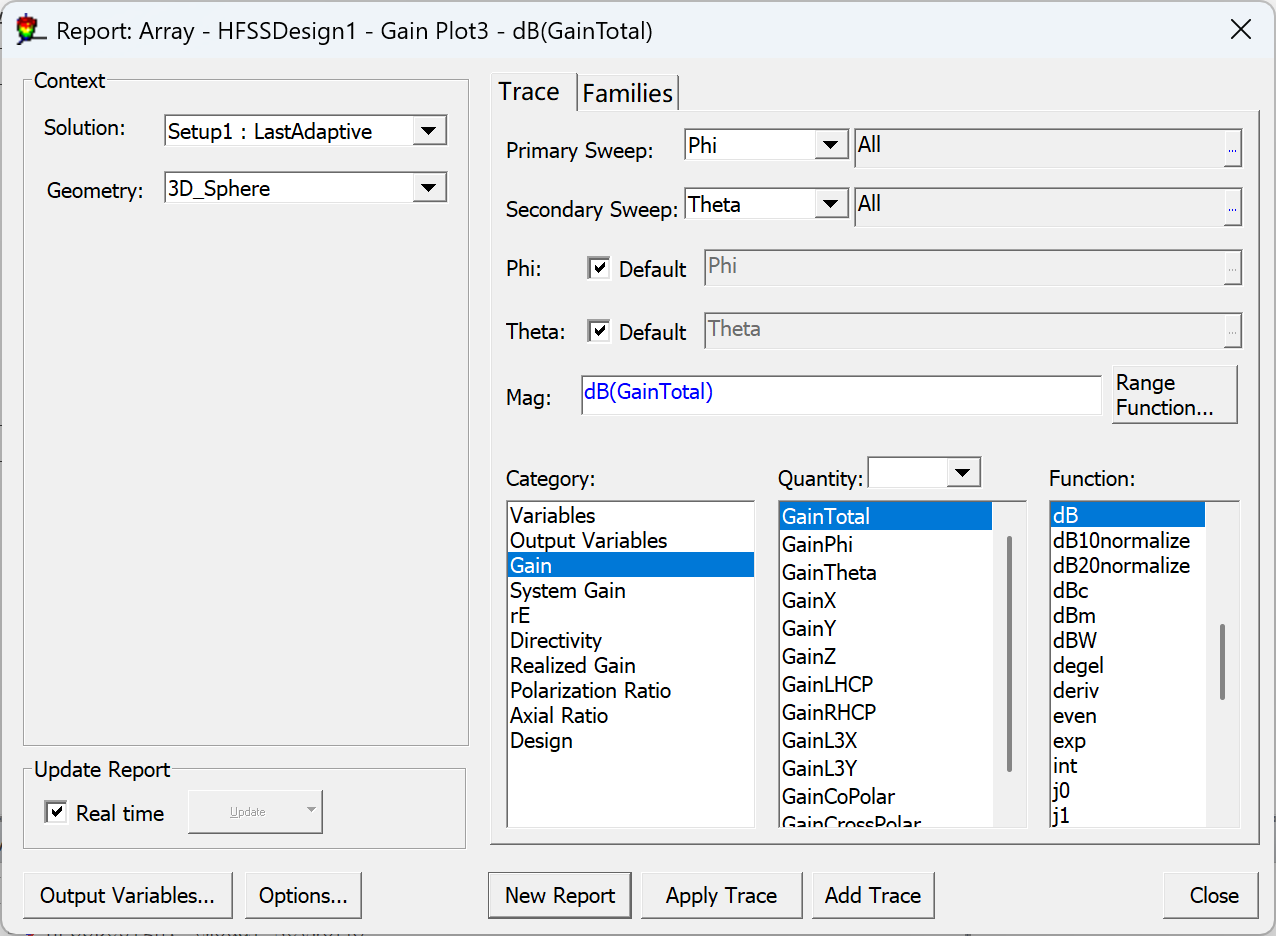
\includegraphics[width=0.6\textwidth]{p28.png}
\caption{3D 辐射方向设置}
\end{figure}

\begin{figure}[H]
\centering
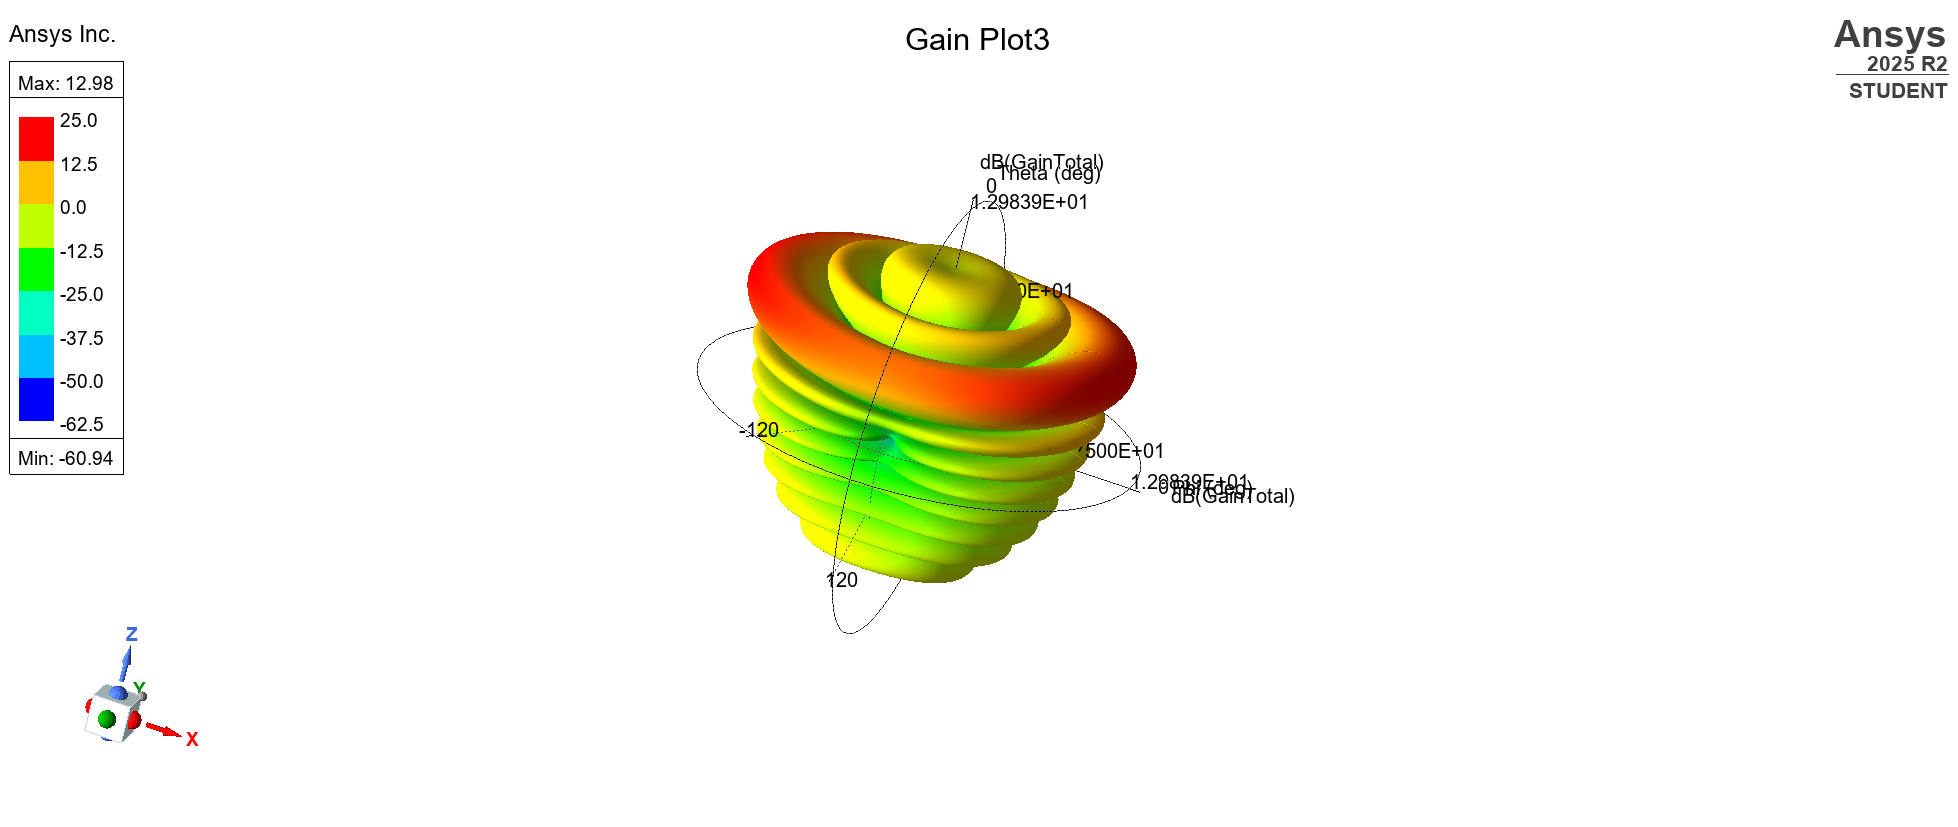
\includegraphics[width=1\textwidth]{p29.png}
\caption{3D辐射方向图}
\label{fig:3d_pattern}
\end{figure}

从 3D 辐射方向图可以看出，该偶极子天线阵的方向性较好，在上半平面增益较大，下半平面增益很小。同时，从天线辐射方向图中可以观察到，其在 Z 方向和 Y 方向上都具有良好的对称性。

\subsection{结果分析总结}

仿真结果准确复现了设计目标：

\begin{enumerate}
\item \textbf{主瓣扫描精度}：天线阵主瓣成功扫描至 $60^\circ$，与理论设计值完全吻合，验证了相位差 $\beta = -90^\circ$ 的正确性。

\item \textbf{增益性能}：在主瓣方向获得了约 12.98 dB 的最大增益，体现了阵列增益的优势。

\item \textbf{无栅瓣设计}：在可见区域内未出现栅瓣，验证了单元间距 $d = \lambda/2 < 2\lambda/3$ 的无栅瓣条件的有效性。

\item \textbf{方向性特征}：XZ 平面具有良好的方向性，XY 平面接近全向，符合均匀线阵的典型辐射特性。

\item \textbf{对称性}：辐射方向图在 Z 方向和 Y 方向上均表现出良好的对称性，说明阵列设计合理。
\end{enumerate}

综上所述，本次实验成功验证了相控阵波束扫描原理和设计方案的正确性。


\section{实验总结与心得体会}

\subsection{实验总结}

本实验基于天线阵理论，成功设计并使用 HFSS 仿真了一个 10 单元偶极子均匀线阵。通过理论计算，我们确定了单元数量（$N=10$）、无栅瓣间距（$d=\lambda/2$）和目标扫描角 $60^\circ$ 所需的激励相位（$\beta=-90^\circ$）等关键参数。

仿真结果准确复现了设计目标：天线阵主瓣成功扫描至 $60^\circ$，获得了约 12.98 dB 的最大增益，且在可见区域内未出现栅瓣。验证了相控阵波束扫描原理和设计方案的正确性。

\subsection{实验心得体会}

本次实验使我获益匪浅，心得体现在三个层面：

\textbf{原理的"具象化"}：我真正将课本上抽象的阵列因子（AF）、波程差和渐变相位 $\alpha$ 等概念，转化为了 HFSS 中可设置、可观察的物理实体和参数。看到主瓣随着相位的变化而扫描，让我对相控阵"移相即扫描"的核心思想有了远超书本的直观理解。

\textbf{工具的"熟练化"}：我熟练掌握了 HFSS 仿真天线阵列的完整流程。特别是学习了如何利用 \keyblue{Antenna Array Setup} 功能高效地实现单元复制和相位加载，而不是手动搭建 10 个单元，这极大提升了仿真效率。

\textbf{设计的"系统化"}：我认识到天线设计是一个系统性工程。单元间距 $d$ 不仅影响主瓣宽度，更要满足无栅瓣条件；而阵列单元数 $N$ 则直接决定了增益和波束宽度。这些参数间的制衡与取舍，让我对工程设计的系统性有了更深的体会。

通过本次实验，我不仅掌握了相控阵天线的设计方法和仿真技巧，更重要的是培养了从理论到实践的完整思维模式，这将对今后的学习和研究产生深远影响。

\end{document}
